\documentclass[../main.tex]{subfiles}

\usepackage{nopageno} %Seitenzahlen auf richtiger Seite 

\usepackage[left=2cm, right=2cm, top=2cm, includehead, includefoot, headheight=17pt]{geometry}

\usepackage[utf8x]{inputenc}
\usepackage[english]{babel}
\usepackage{amsmath,amssymb,amsthm}
\usepackage{framed}
\usepackage{wasysym}
\usepackage[T1]{fontenc} %Silbentrennung 
\usepackage{color} %Farbe
\usepackage{graphicx}
\usepackage{float}%Grafik am gleichen Ort plazieren
%pdf. png. einfach eingliedern
\usepackage{subfigure} %Grafiken nebeneinander
\usepackage{pdfpages}
\usepackage{ulem} 	%\uuline{urgent}    % doppelt unterstreichen
%\uwave{boat}      % unterschlängeln
%\sout{wrong}       % durchstreichen
%\xout{removed}     % ausstreichen mit //////.

\usepackage{tikz}
\usetikzlibrary{trees}
\usetikzlibrary{plotmarks}
\usetikzlibrary{angles,quotes,babel}
\usetikzlibrary{shadings}
\usetikzlibrary{patterns}
\usetikzlibrary{matrix}
\usetikzlibrary{arrows}
\usetikzlibrary{calc}

\usepackage{pgfplots}
\usepackage{pgf-pie}
\pgfplotsset{compat=1.10}
\usepgfplotslibrary{statistics}
\usepgfplotslibrary{fillbetween}

\usepackage{tkz-euclide}
\usepackage{enumerate}
\usepackage{stmaryrd}
\usepackage{tabularx}
\usepackage{wrapfig}
\usepackage{epsdice}
\usepackage{multirow}
\usepackage{rotating}
\usepackage{pdflscape}
\usepackage{fancyhdr}

\pagestyle{fancy} %eigener Seitenstil
\fancyhf{} %alle Kopf- und Fußzeilenfelder bereinigen
\fancyhead[L]{} %Kopfzeile links
\fancyhead[C]{} %zentrierte Kopfzeile
\fancyhead[R]{} %Kopfzeile rechts
\renewcommand{\headrulewidth}{0.4pt} %obere Trennlinie
\fancyfoot[C]{\thepage} %Seitennummer
\renewcommand{\footrulewidth}{0.4pt} %untere Trennlinie

% Number spaces 
\newcommand{\CC}{\ensuremath{\mathbb{C}}}
\newcommand{\RR}{\ensuremath{\mathbb{R}}}
\newcommand{\QQ}{\ensuremath{\mathbb{Q}}}
\newcommand{\ZZ}{\ensuremath{\mathbb{Z}}}
\newcommand{\NN}{\ensuremath{\mathbb{N}}}
\newcommand{\LL}{\ensuremath{\mathbb{L}}}
\newcommand{\DD}{\ensuremath{\mathbb{D}}}
\newcommand{\WW}{\ensuremath{\mathbb{W}}}

%draw chemestry molecules 
\usepackage{chemfig} % https://mirror.ox.ac.uk/sites/ctan.org/macros/generic/chemfig/

\newcommand\vv[1]{%
	\begin{tikzpicture}[baseline=(arg.base)]
		\node[inner xsep=0pt] (arg) {$#1$};
		\draw[line cap=round,line width=0.45,->,shorten >= 0.2pt, shorten <= 0.7pt] (arg.north west) -- (arg.north east);
	\end{tikzpicture}%
} %command will render \vv{x} with an arrow aboth 

\renewcommand{\labelenumi}{\roman{enumi})}

\DeclareMathOperator{\ggT}{ggT}
\DeclareMathOperator{\sign}{sign}

%sections
\theoremstyle{plain}
\newtheorem{Thm}{Theorem}[section]
\newtheorem{Def}[Thm]{Definition}
\newtheorem{Prop}[Thm]{Proposition}

\theoremstyle{definition}
\newtheorem{lemma}[Thm]{Lemma}
\newtheorem{corollary}[Thm]{Corollary}
\newtheorem{claim}[Thm]{Claim}
\newtheorem{Proof}[Thm]{Proof}
\newtheorem{Ex}[Thm]{Example}

\newtheorem{Exercise}{ex}[section] %follow proper enum
\newtheorem{ex}[Exercise]{Exercise}
\newtheorem{Solution}{sol}[section]
\newtheorem{sol}[Solution]{Solution}

\theoremstyle{remark}
\newtheorem{remark}[Thm]{Remark} % follows thm enum

\newtheorem{comment}{Comment}[section] %follow comment enum
\newtheorem{notation}[comment]{Notation}
\newtheorem{reasoning}[comment]{Reasoning}
\newtheorem{Intpr}[comment]{Interpretation}

%some premmade with title (uterwise use \textbf{Title} ...)
\newenvironment{ThmWithTitle}[1]{%
	\begin{Thm}[\textbf{#1}]}{\end{Thm}}
\newenvironment{PropWithTitle}[1]{%
	\begin{Prop}[\textbf{#1}]}{\end{Prop}}
\newenvironment{ExWithTitle}[1]{%
	\begin{Ex}[\textbf{#1}]}{\end{Ex}}
\newenvironment{DefWithTitle}[1]{%
	\begin{Def}[\textbf{#1}]}{\end{Def}}
\newenvironment{RemarkWithTitel}[1]{%
	\begin{remark}[\textbf{#1}]}{\end{remark}}

%format of paragraph 
\renewcommand\paragraph{\@startsection{paragraph}{4}{\z@}%
	{-2.5ex\@plus -1ex \@minus -.25ex}%
	{1.25ex \@plus .25ex}%
	{\normalfont\normalsize\bfseries}}
\makeatother
\setcounter{secnumdepth}{4} % how many sectioning levels to assign numbers to
\setcounter{tocdepth}{4}    % how many sectioning levels to show in ToC

\newcounter{row} 
\renewcommand\therow{\alph{row}} %hier a,b,c etc. def und mit therow abrufbar

\newenvironment{aufz}
{\setcounter{row}{0}%
	\par\noindent\tabularx{\linewidth}[t]
	{\cdot{20}{>{\stepcounter{row}\makebox[1.5em][l]{\therow)\hfill}}X}} %bis max 20 Elemente nebeinander
}
{\endtabularx}


%biblio
\usepackage[]{biblatex}
\addbibresource{referenzenma.bib} 

%glossary
\usepackage{glossaries}
\usepackage{import}


\usepackage{rotating} % Include this package in the preamble

\newglossaryentry{hexokinase}{
	name={Hexokinase},
	description={An enzyme that catalyzes the phosphorylation of glucose to glucose-6-phosphate, the first step in glycolysis.}
}

\newglossaryentry{pyruvate}{
	name={Pyruvate},
	description={A three-carbon molecule that is the end product of glycolysis.}
}

\newglossaryentry{fanaerorg}{
	name={Facultative Anaerobic Organism},
	description={A organism that is able to produce ATP by anerobic respiration if oxygen is present, but is also capable of switching to fermentation if oxygen is absent}
}

\newglossaryentry{pdh}{
	name={pyruvate dehydrogenase complex (PDH complex or PDC)},
	description={a multi-enzyme complex that catalyzes the conversion of pyruvate into acetyl-CoA, linking glycolysis to the citric acid cycle},
	sort=pyruvatedehydrogenase
}

\newglossaryentry{pyruvatetranslocase}{
	name={pyruvate translocase},
	description={a transport protein located in the inner mitochondrial membrane that facilitates the import of pyruvate from the cytosol into the mitochondrial matrix for further metabolic processing},
	sort=pyruvatetranslocase
}

\newglossaryentry{lipoyllysine}{
	name={lipoyllysine},
	description={a covalent complex of lipoic acid attached via an amide bond to the $\epsilon$-amino group of a lysine residue. It serves as a swinging arm in multi-enzyme complexes like the pyruvate dehydrogenase complex, transferring reaction intermediates between active sites. It has \textbf{two thiol groups} that can undergo reversible oxidation to a disulfid bond.},
	sort=lipoyllysine
}

\newglossaryentry{tpp}{
	name={thiamine pyrophosphate (TPP)},
	description={a coenzyme derived from vitamin B1, essential in decarboxylation reactions such as those in the pyruvate dehydrogenase complex. It stabilizes carbanion intermediates via its thiazolium ring},
	sort=thiaminepyrophosphate
}

\newglossaryentry{succinatedehydrogenase}{
	name={succinate dehydrogenase},
	description={an enzyme that catalyzes the oxidation of succinate to fumarate in the citric acid cycle (step 6). It is also part of Complex II in the electron transport chain, linking the TCA cycle with oxidative phosphorylation by transferring electrons from FADH2 to ubiquinone (coenzyme Q)},
	sort=succinatedehydrogenase
}

\newglossaryentry{bileacids}{
	name={bile acids},
	description={amphipathic molecules derived from cholesterol that aid in the digestion and absorption of dietary fats by emulsifying lipids and facilitating micelle formation. They are synthesized in the liver, stored in the gallbladder, and released into the small intestine. Bile acids are also involved in cholesterol excretion and undergo enterohepatic circulation},
	sort=bileacids
}

\newglossaryentry{carnitine}{
	name={Carnitine},
	description={ammonium compound that plays a crucial role in the transport of long-chain fatty acids into the mitochondrial matrix for $\beta$-oxidation. Carnitine enabling them to cross the inner mitochondrial membrane via the carnitine shuttle system},
	sort=carnitine
}


\newglossaryentry{plp}{
	name={pyridoxal phosphate (PLP)},
	description={A cofactor derived from vitamin B\textsubscript{6}, essential for amino acid metabolism. PLP is involved in transamination, decarboxylation, and deamination reactions}
}

\newglossaryentry{anabolism}{
	name={Anabolism},
	description={Metabolic pathways that build complex molecules from simpler ones, requiring an input of energy.}
}

\newglossaryentry{atp}{
	name={ATP (Adenosine Triphosphate)},
	description={The primary energy currency of the cell, used to power many cellular processes. Its hydrolysis releases heat but not energy, while the transfer of phosphate leads to a higher state in free energy of the substrate.}
}

\newglossaryentry{catabolism}{
	name={Catabolism},
	description={Metabolic pathways that break down complex molecules into simpler ones, releasing energy.}
}

\newglossaryentry{coupledreactions}{
	name={Coupled Reactions},
	description={Two chemical reactions linked together, where an energetically favourable reaction (e.g., ATP hydrolysis) provides the energy to drive an energetically unfavourable reaction.}
}

\newglossaryentry{electroncarrier}{
	name={Electron Carrier},
	description={Molecules that can accept and donate electrons, facilitating the transfer of energy in redox reactions (e.g., NAD+, FAD).}
}

\newglossaryentry{glycolysis}{
	name={Glycolysis},
	description={A universal metabolic pathway that breaks down glucose into pyruvate, producing a net gain of ATP and NADH.}
}

\newglossaryentry{metabolism}{
	name={Metabolism},
	description={The sum of all chemical reactions that occur within a living organism to maintain life.}
}

\newglossaryentry{oxidation}{
	name={Oxidation},
	description={The loss of electrons or an increase in oxidation state of a molecule. Often involves the addition of oxygen or removal of hydrogen.}
}

\newglossaryentry{phosphorylation}{
	name={Phosphorylation},
	description={The addition of a phosphate group to a molecule, often increasing its energy or altering its activity.}
}


\newglossaryentry{reduction}{
	name={Reduction},
	description={The gain of electrons or a decrease in oxidation state of a molecule. Often involves the addition of hydrogen or removal of oxygen.}
}

\newglossaryentry{secondlaw}{
	name={Second Law of Thermodynamics},
	description={States that the total entropy of an isolated system can never decrease over time.}
}

\newglossaryentry{enthalpy}{
	name={Enthalpy (H)},
	description={A thermodynamic quantity representing the total heat content of a system. In biochemistry, enthalpy changes (\(\Delta H\)) are associated with bond formation and breaking, influencing biochemical reactions and energy transfer.}
}

\newglossaryentry{entropy}{
	name={Entropy},
	description={A measure of the disorder or randomness of a system. The second law of thermodynamics states that the total entropy of an isolated system tends to increase over time.}
}

\newglossaryentry{exergonicreaction}{
	name={Exergonic Reaction},
	description={A chemical reaction that releases energy (has a negative \( \Delta G \)) and is therefore favorable. }
}

\newglossaryentry{freeenergy}{
	name={Free Energy (G)},
	description={The portion of a system's energy that is available to do useful work.}
}


\newglossaryentry{kinase}{
	name={Kinase},
	description={An enzyme that catalyzes the transfer of phosphate groups from high-energy donor molecules, such as ATP, to specific substrates, a process known as phosphorylation.}
}

\newglossaryentry{phosphatase}{
	name={Phosphatase},
	description={An enzyme that removes phosphate groups from proteins or other molecules, a process known as dephosphorylation, which often regulates cellular activity.}
}

\newglossaryentry{dehydrogenase}{
	name={Dehydrogenase},
	description={An enzyme that catalyzes the removal of two hydrogen atoms from a substrate, typically transferring them to an electron acceptor such as NAD$^+$ or FAD. Dehydrogenases play a crucial role in metabolic pathways like glycolysis and the citric acid cycle.}
}

\newglossaryentry{oxidase}{
	name={Oxidase},
	description={An enzyme that catalyzes oxidation reactions, using molecular oxygen (O$_2$) as the electron acceptor without incorporating it into the substrate. Oxidases are involved in various biological oxidation processes, including those in the electron transport chain.}
}

\newglossaryentry{oxygenase}{
	name={Oxygenase},
	description={An enzyme that catalyzes the incorporation of oxygen atoms from molecular oxygen (O$_2$) into a substrate. Oxygenases are classified into monooxygenases and dioxygenases, which incorporate one or two oxygen atoms, respectively, and are essential in metabolic pathways like drug metabolism and biosynthesis.}
}

\newglossaryentry{reducingequivalent}{
	name={Reducing Equivalent},
	description={A unit of reducing power in biochemical redox reactions, referring to the transfer of one electron (or its equivalent as a hydrogen atom or hydride ion). Reducing equivalents are carried by molecules such as NADH, NADPH, and FADH$_2$, playing a crucial role in cellular respiration and biosynthetic pathways.}
}

\newglossaryentry{niacin}{
	name={Niacin (Vitamin B3)},
	description={A water-soluble B vitamin essential for energy metabolism, DNA repair, and cell signaling. Niacin is a precursor to the coenzymes NAD$^+$ and NADP$^+$, which are crucial for redox reactions in cellular respiration and biosynthetic pathways}
}

\newglossaryentry{arsenatepoisoning}{
	name={Arsenate Poisoning},
	description={A toxic condition caused by exposure to arsenate (AsO$_4^{3-}$), which disrupts cellular metabolism by mimicking phosphate. Arsenate can uncouple oxidative phosphorylation by substituting for inorganic phosphate glycolisys or ATP synthesis, leading to decreased ATP production and cellular toxicity. Symptoms include nausea, vomiting, neurological disturbances, and multi-organ failure in severe cases.}
}

\newglossaryentry{nad}{
	name={NAD$^+$ (Nicotinamide Adenine Dinucleotide)},
	description={A coenzyme involved in redox reactions, serving as an electron carrier in cellular respiration. NAD$^+$ is reduced to NADH, which donates electrons to the electron transport chain for ATP production.}
}

\newglossaryentry{nadp}{
	name={NADP$^+$ (Nicotinamide Adenine Dinucleotide Phosphate)},
	description={A phosphorylated form of NAD$^+$ that functions as an electron carrier, primarily in anabolic pathways such as fatty acid and nucleotide biosynthesis. NADP$^+$ is reduced to NADPH, which provides reducing power for biosynthetic reactions.}
}

\newglossaryentry{fad}{
	name={FAD (Flavin Adenine Dinucleotide)},
	description={A redox-active coenzyme associated with various enzymes, particularly in the electron transport chain and fatty acid oxidation. FAD is reduced to FADH$_2$, which donates electrons to the respiratory chain.}
}

\newglossaryentry{fmn}{
	name={FMN (Flavin Mononucleotide)},
	description={A coenzyme derived from riboflavin (vitamin B2) that acts as a prosthetic group in various oxidoreductases, including NADH dehydrogenase in the electron transport chain. FMN is involved in redox reactions, cycling between oxidized and reduced states.}
}


\newglossaryentry{flavoprotein}{
	name={Flavoprotein},
	description={A protein that contains a flavin coenzyme, such as FAD or FMN, as a prosthetic group}
}

\newglossaryentry{ubiquinone}{
	name={Ubiquinone (Coenzyme Q)},
	description={A lipid-soluble electron carrier in the electron transport chain, transferring electrons between complex I/II and complex III. Ubiquinone exists in oxidized (Q), semiquinone (Q$^-$), and reduced (QH$_2$) forms.}
}



\makeglossaries

\begin{document}
	
\section{Catabolism}
The catabolism of proteins, fats, and carbohydrates can be divided into 3 stages: 
\begin{itemize}
	\item Stage 1: Oxidation of fatty acids, glucose, and some amino acids yield acetyl-CoA.
	\item Stage 2: Oxidation of acetyl groups in the citric acid cycle includes 4 steps in which electrons are abstracted. 
	\item Stage 3: Electrons carried by NADH and FADH2 are funneled into a chain of mitochondrial (in bacteria plasma membrane-bound) electron carriers - the repiratory chain -ultimately reducing O2 to H2O. This electron flow drives the production of ATP. 
\end{itemize}

\begin{figure}[H]
	\centering
	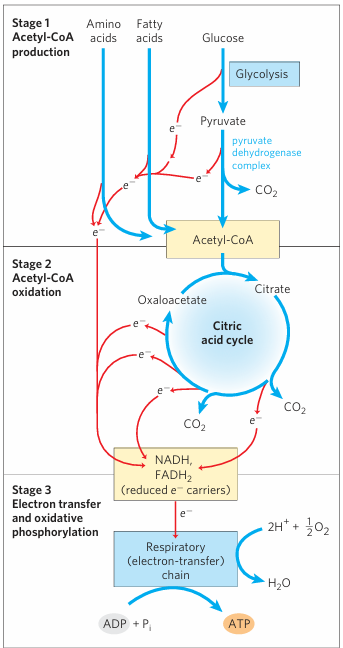
\includegraphics[height = 14cm]{gen1}
	\caption{3 stages of cellular respiration}
\end{figure}
	
\subsection{Glycolysis}
\textbf{D-Glucose} is the major nutrient for a wide range of organisms. It can be stored by cells in the form of polymers and used upon need to generate ATP. \\
\\
In glycolysis (from the Greek \textit{glycus}, "sugar", and \textit{lysis}, "spliting") a molecule of \textbf{glucose} is degraded in a serie of enzyme-catalized reactions \textbf{to two} molecules of \textbf{pyruvate}.
\begin{figure}[H]
	\centering
	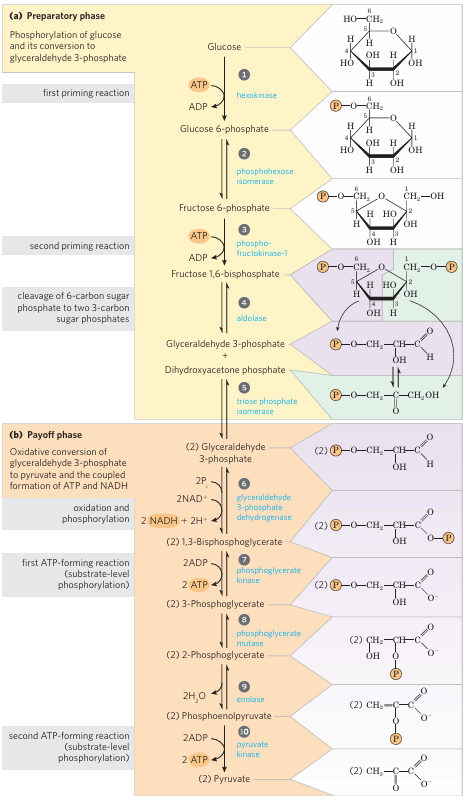
\includegraphics[width = 0.6 \textwidth]{glycolysis_gen}
	\caption{Glycolysis}
\end{figure}
\begin{itemize}
	\item \textbf{Glucose} + 2ADP + 2NAD+ + 2Pi => \textbf{2 Pyruvate + 2ATP + 2NADH} + 2 H+ + 2 H2O
\end{itemize}

\paragraph{Carbon labeling}
Note when labeling GA3P the number do not correspond to the same numbers from the fructose compound. \textit{One always follows the normal rules}
\begin{figure}[H]
	\centering
	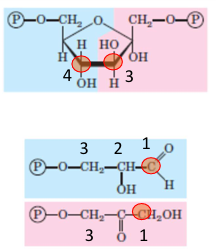
\includegraphics[height = 5cm]{labeling}
	\caption{Carbon labeling}
\end{figure}

Glycolysis can be dived in two stages the preparation phase and the payoff phase. 

\subsubsection{Stage 1, Preparation Phase}
In the preparation phase glucose gets \textbf{trapped} inside the cell, "\textbf{activated}", and \textbf{broken down} into smaller components.  
\paragraph{Step1: Posphorylation of Glucose}
\textbf{D-Glucose} moves into the cell with the help of a \textbf{membrane transporter}. Once in the cytoplasma it undergoes phosporylation by \textbf{hexokinase} to produce \textbf{Glucose 6-phosphate}. This has two consequences: 
\begin{itemize}
	\item \textbf{No backsies}: Glucose 6-phosphate is structurally different and thus can not be transported out by the same membrane transporter. 
	\item \textbf{More reactive}: The substitution of the hydroxy group with the phosphate group (2 additional charges, etc.) makes the molecule more reactive. But this has to be payed by the \textbf{investment} of 1 ATP molecule.
\end{itemize}

\begin{figure}[H]
	\centering
	\subfigure[Step 1]{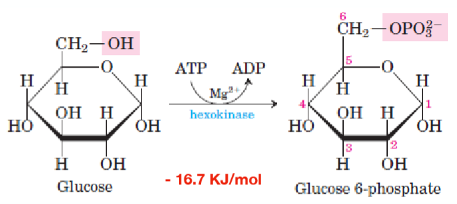
\includegraphics[width = 0.6 \textwidth]{S1}}
	\subfigure[Hexokinase]{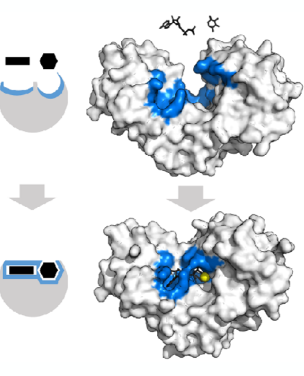
\includegraphics[width = 0.25 \textwidth]{HK}\label{HK}}
	\caption{Posphorylation of Glucose}
\end{figure}

\begin{RemarkWithTitel}{Hexokinase (HK)}
	\gls{hexokinase} is an enzyme that phosphorylates hexoses (like glucose) using ATP. Like most kinases it requires the presence of the cofactor Mg2+ in the active site. \\
	The movement of Glucose into HK active site causes a conformational change whereby two HK lobes rotate by 12 degrees (10 \AA) creating an \textbf{induced fit}. This makes the \textbf{carbon 6 oriented towards ATP} and squeezes out water molecules. (see fig. \ref{HK}) 
\end{RemarkWithTitel}

\paragraph{Step2: Isomerization}
In the second step, the enzyme \textbf{phospho-glucose isomerase} also transforms aldose (glucose) into ketose (fructose). This is done to create more symmetry in preparation for step 3. 

\begin{figure}[H]
	\centering
	\subfigure[6 to 5 ring]{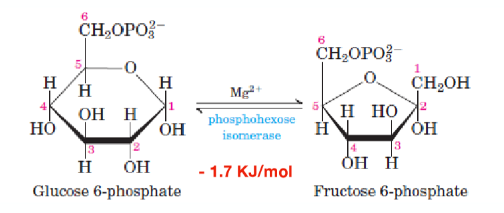
\includegraphics[width = 0.6 \textwidth]{S2_1}}
	\subfigure[aldose to ketose]{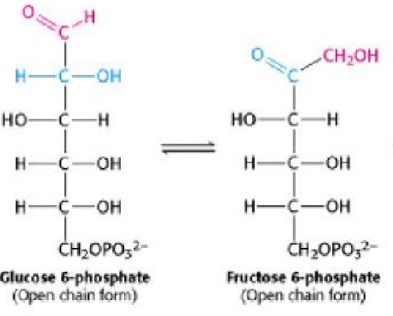
\includegraphics[width = 0.3 \textwidth]{S2_2}}
	\caption{Isomerization}
\end{figure}

\paragraph{Step3: Second phosphorylation}
The enzyme \textbf{phospho-fructo kinase-1 (PFK-1)} turns Fructose 6-phophate into Fructiose 1,6-biphosphate, completing the symmetry and making the compound even more reactive. This is again paid with the \textbf{investment of 1 ATP}. (see fig. \ref{S3})\\
\\
Note, that \textbf{this step commits the sugar to glycolysis}. This is why \textbf{PFK-1 is a highly regulated enzyme} where its activity is modified according to cellular concentration of ATP, ADP, and AMP. (\textbf{ATP inhibits - AMP stimulates}). 

\paragraph{Step4: Breakdown of Fructose 1,6-biphosphate}
\textbf{Aldolase} catalyses the breakdown of Fructose 1,6-biphosphate into 2 different three-carbon molecules (\textbf{GA3P and DHAP}). 
\begin{figure}[H]
	\centering
	\subfigure[creation of perfect symmetry]{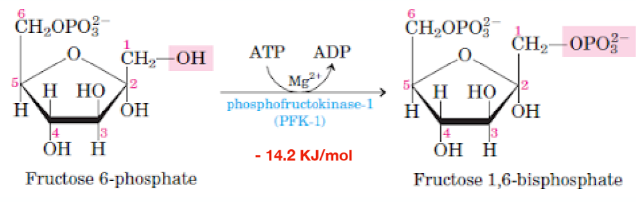
\includegraphics[width = 0.48\textwidth]{S3}\label{S3}}
	\subfigure[breakdown]{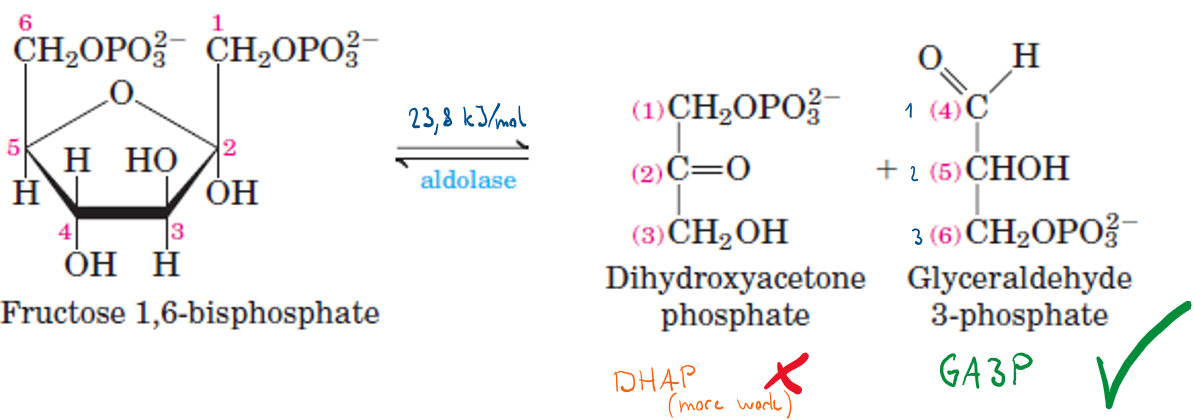
\includegraphics[width = 0.49 \textwidth]{S4}}
	\caption{Step3 and Step4}
\end{figure}
GA3P feeds directely in the glycolytic pathway without any further change while DHAP needs to be first transformed.  This is archived by Step5. 

\paragraph{Step5: Isomerisation of DHAP to GA3P}
\textbf{Triose phosphate isomerase (TPI or TIM)} catalyses the rapid and reversible conversion of DAHP to GA3P, ketone to aldehyde. This happens via an intramolecular redox reactimon where \textbf{an hydrogen is transferred from C1 to C2}.
\begin{figure}[H]
	\centering
	\subfigure[Step5]{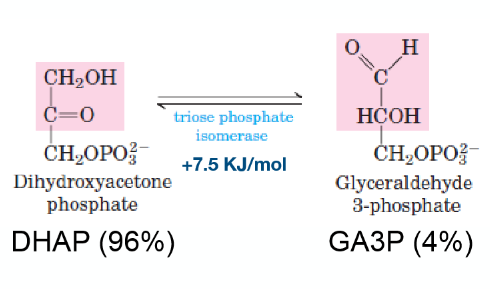
\includegraphics[width = 0.4 \textwidth]{S5_1}}
	\subfigure[Mechanism of TIP]{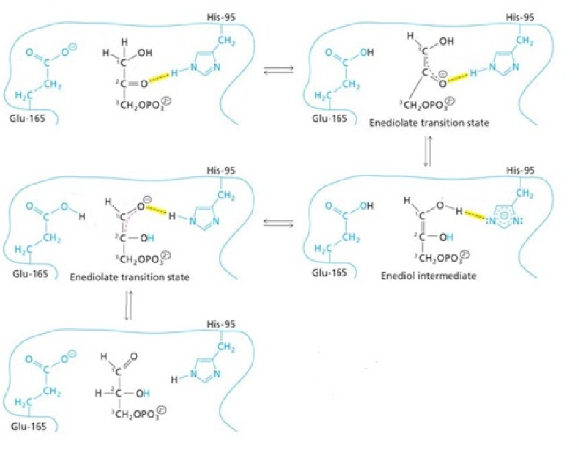
\includegraphics[width = 0.55 \textwidth]{S5_2}}
	\caption{Isomerisation of DHAP to GA3P}
\end{figure}
Even though TIP increases the rate by 10 billion fold the equilibrium still lies on the unwanted side of DHAP (the \textbf{reaction is unfavorable, endergonic}). But since the reaction is coupled to an exergonic reaction that removes GA3P, thus via le chatelier \textbf{the reactions shifts to the side of the product GA3P}.  

\subsubsection{Stage 2, Payoff Phase}
In the payoff phase the components from the stage 1 get \textbf{oxidized} in order to produce ATP, NADH, and pyruvat. 

\paragraph{Step6: Conversion of GA3P to 1,3-BPG}
GA3P is converted into 1,3-biphosphoglycerate (1,3-BPG) by the enzyme glyceraldehyde 3-phophate \textbf{dehydrogenase (GAPDH)}. Note this reaction produces NADH, which can later be oxidized.  
\begin{figure}[H]
	\centering
	\subfigure[Step6]{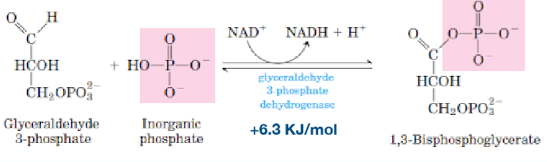
\includegraphics[width = 0.4 \textwidth]{S6_1}}
	\subfigure[Mechanism of GAPDH]{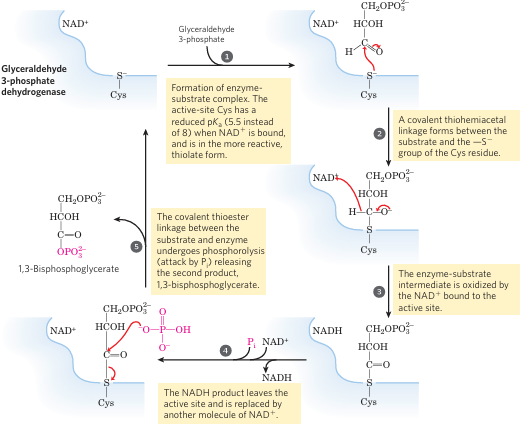
\includegraphics[width = 0.4 \textwidth]{S6_2}}
	\caption{Conversion of GA3P to 1,3-BPG}
\end{figure}

\paragraph{Step7: Phosphotransfer from 1,3-BPG to ADP}
Step7 is the \textbf{break-even point}. 1, 3-BPG is used as a phophate doner to ADP. This reaction is catalyzed by \textbf{glycerophophate kinase} and produces 3-Phophoglycerate and ATP. (see fig. \ref{S7})

\paragraph{Step8: Conversion to 2-Phophopglycerate}
\textbf{Phosphoglycerate mutase} catalyses the transfer of the phosphate group from C3 of 3-phosphoglycerate to C2 to form 2-phosphoglycerate. 

\begin{figure}[h!]
	\centering
	\subfigure[Break-Even point]{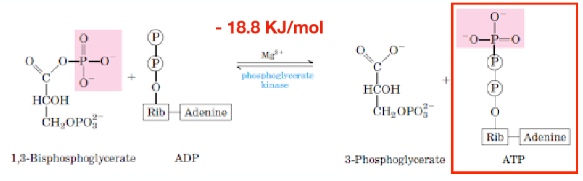
\includegraphics[width = 0.49 \textwidth]{S7}\label{S7}}
	\subfigure[Repositioning of Phosphate group]{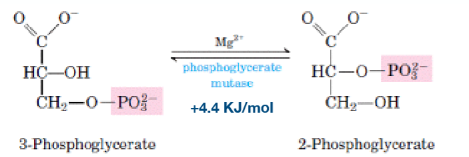
\includegraphics[width = 0.48 \textwidth]{S8}}
	\caption{Step7 and Step8}
\end{figure}

\paragraph{Step9: Conversion to Phophoenolpyruvate (PEP)}
\textbf{Enolase} converts 2-phosphoglycerate into phosphoenolpyruvate (PEP). This \textbf{dehydration reaction increases the phosphoryltransfer potential} of the molecule.

\paragraph{Step10: Conversion to Pyruvate}
The phosphoryltransfer potential of \textbf{PEP} is exploited to create ATP and pyruvate. The enzyme \textbf{pyruvate kinase} catalyses the phosphoric transfer. At this point we have gained a \textbf{total of 2 ATP and 2 NADH}. 
\begin{figure}[h!]
	\centering
	\subfigure[Dehydration by enolase]{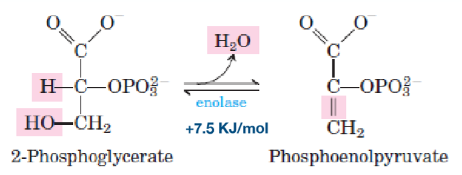
\includegraphics[width = 0.45 \textwidth]{S9}\label{S9}}
	\subfigure[Gain of 2 ATP and 2 Pyruvate]{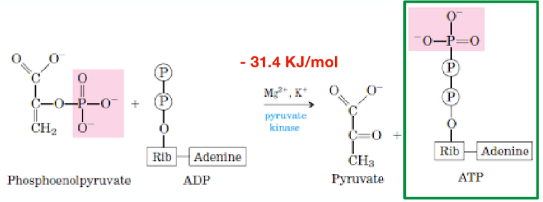
\includegraphics[width = 0.45 \textwidth]{S10}}
	\caption{Step9 and Step10}
\end{figure}

\subsubsection{The fates of Pyruvate}
\gls{pyruvate} is a three-carbon molecule that is the end product of glycolysis.

\begin{figure}[H]
	\centering
	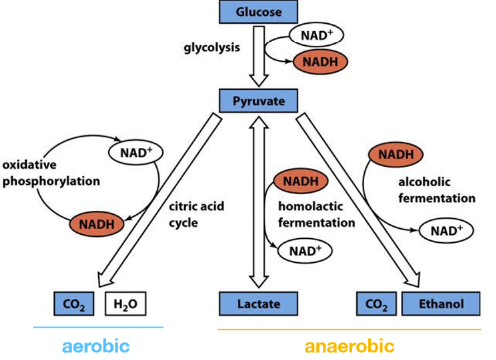
\includegraphics[width = 0.7 \textwidth]{fate_of_pyruvate}
	\caption{The fates of Pyruvate}
\end{figure}

\begin{DefWithTitle}{Facultative Anaerobic Organism}
	A \gls{fanaerorg} is able to produce ATP by anerobic respiration if oxygen is present, but is also capable of switching to fermentation if oxygen is absent. For example E.coli or some muscle cells (temporarily in humans). 
\end{DefWithTitle}

\begin{RemarkWithTitel}{Soy Sauce}
	Soy sauce is produced by \textbf{fermenting a salted mixture of soy beans}. Soybeans contain starch whcih will be broken down to glucose and then degradated via glycolysis to pyruvate. And the fermented in the absence of oxygen. However \textbf{if oxygen were present} pyruvate would be oxydized to acetyl-CoA entering the citric acid cycle. But some a\textbf{cetyl-CoA would get hydrolyzed to acetic acid (vinegar)} which would result in a undesired strong vinegar taste.
\end{RemarkWithTitel}

\paragraph{Ethanol Fermentation}
\textbf{Yeast} and sveral bacteria utilise ethanol (alcoholic) fermentation to \textbf{regenerate NAD+} and to transform pyruvate into \textbf{ethanol and carbon dioxide}.\\
\\
In a first step \textbf{pyruvate decarboxylase} catalyses a decarboxylation reaction. The enzymes needs the\textbf{ coenzyme TPP}, a vitamin B1 derivative, and cofactor Mg2+ 
\begin{itemize}
	\item Note, that the \textbf{C3 \& C4 carbons of glucose will be cut away} in form of CO2. (glucose -> 2 pyruvate)
\end{itemize}
In the second step \textbf{alcohol dehydrogenase} will regenerate NAD+ in reducing acetaldehyde to ethanol. Note alcohol dehydrogenase conatins a \textbf{zinc ion} in the active site to help polarize the carbonyl double bond that promotes hydride (negative charged hydrogen) transfer from NADH. 

\begin{figure}[H]
	\centering
	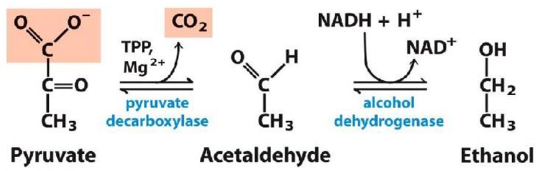
\includegraphics[width = 0.6 \textwidth]{ethanol}
	\caption{Ethanol Fermentation}
\end{figure}

\begin{itemize}
	\item Glucose + 2ADP + 2Pi => 2 Ethanol + \textbf{2ATP} + 2 CO2 + 2 H2O
\end{itemize}

\paragraph{Lactic Fermentation}
\textbf{Many prokaryotic and eukaryotic} organisms can use lactic fermentation. Like ethanol fermentation it is nessesary to \textbf{regenerate NAD+}. Lactic fermentation is catalysed by \textbf{lactate dehydrogenase (LHD)}. 

\begin{figure}[H]
	\centering
	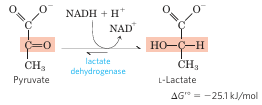
\includegraphics[width = 0.6 \textwidth]{lactic}
	\caption{Lactic Fermentation}
\end{figure}

\begin{RemarkWithTitel}{Cancer, PET scan}
	Cancer cells often rely on aerobic glycolysis, known as the\textbf{ Warburg effect}, where they preferentially use glycolysis followed by lactic acid fermentation, even in the presence of oxygen. This allows them to rapidly generate ATP and biosynthetic precursors for growth.\\
	Positron Emission Tomography (PET scans) exploit this metabolic shift by using \textbf{fluorodeoxyglucose (FDG)}, a radiolabeled \textbf{glucose analog, that will not undergo full gylcolysis (thus accumulate)}. Since cancer cells have a higher glucose uptake due to increased glycolysis, they accumulate FDG, which emits positrons detectable by \textbf{PET imaging}.
\end{RemarkWithTitel}


\subsection{TCA cycle}
In aerobic organisms, glucose and other sugars, fatty acids, and most amino acids are ultimately oxidized to CO2 and H2O via the citric cycle and the respiratory chain. 

\begin{RemarkWithTitel}{TCA cycle}
	The TCA cycle (TCA = tricarboxylic acid) is also called \textbf{Krebs cylce} or \textbf{citric acid cycle}
\end{RemarkWithTitel}

Before entering the citric acid cycle, the carbon sekeleton of sugars and fatty acids are degraded to the acetyl group of acetyl-CoA

\paragraph{Pyruvate => Acetyl-CoA}

\begin{RemarkWithTitel}{\gls{pyruvatetranslocase}}
	Once produced in the cytosol, pyruvate migrates into the mitochondrial matrix through the action of pyruvate translocases that mediate the transport of pyruvate across mitochondrial membranes. 
\end{RemarkWithTitel}

In the mitochondria pyruvate is converted to acedtyl-CoA in order to enter the TCA cylce. This is done by the \textbf{pyruvate dehydrogenase complex} which catalyses an \textbf{oxidative decarboxylation}, an \textbf{irreversible} oxidation process in which the carbonyl group is removed from pyruvate as an molecule of CO2. 

The combined dehydogenation and decarboxylation of pyruvate requires the sequental action of 3 different enzymes:  
\begin{itemize}
	\item E1 - Pyruvate dehydogenase: Catalyses the redox-decarbocylation reaction. 
	\item E2 - Dihydrolipoyl transacetylase: Catalyses the transfer of the acetyl group.
	\item E3 - Dihydrolipoyl dehydrogenase: Reforms the oxidised version of lipoamide. 
\end{itemize}
\noindent
Moreover 5 different co-enzymes are acting across the 5 different steps (see fig. \ref{TCA0_2}): 
\begin{itemize}
	\item Step 1: Pyruvate reacts with the coenzyme \textbf{gls{tpp}}  bound to E1, and undergoes decarboxylation to the hydroxyethyl derivative.    
	\item Step 2: E1 also carries out step 2, transferring 2 electrons and then the acetyl group (oxidized form of hydrocyenthanyl group) from TPP to the oxidized and then reduced form of the coenzyme \textbf{\gls{lipoyllysine}} of E2. This reduces the disulfid bond of lipoyllysine and binds the acetyl group covelentely as a thiolester. \\
	\textit{Note that lipoyllysine has two thiol groups that can undergo reversible oxidation to a disulfid bond, similar to that between two Cys residues in a protein. Therefore it can serve as both electron carrier and as an acyl carrier.}
	\item Step 3: The acetate is \textbf{trans-estrified} to the SH group of \textbf{CoA-SH}. 
	\item Step 4: liopic acid is oxidised to to refom the S-S bond and 2 hydrate groups are transferred to \textbf{FAD}, the coenzyme bound to E3. FAD is reduced to FADH2. 
	\item Step 5: FAD is regenerated, transferring electrons to the coenzyme \textbf{NAD+} to produce NADH and H+. 
\end{itemize}  
\begin{figure}[H]
	\centering
	\subfigure[Overall reaction]{
		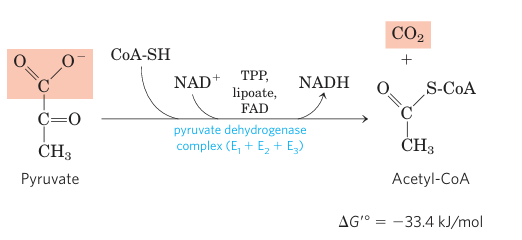
\includegraphics[width=0.45\textwidth]{TCA0_1}
	}
	\subfigure[PDH complex]{
		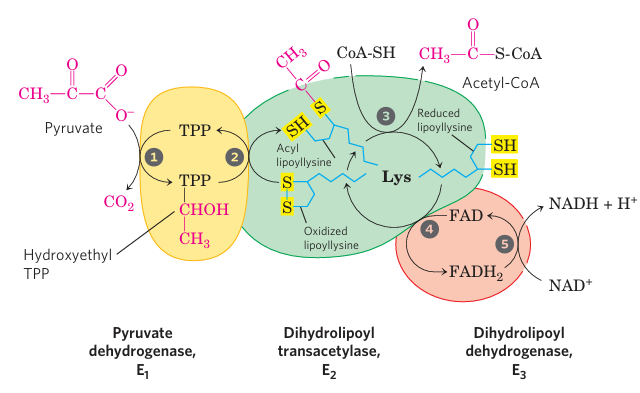
\includegraphics[width=0.45\textwidth]{TCA0_2}
		\label{TCA0_2}
	}
	\caption{Pyruvate + CoA-SH + NAD+ => Acetyl-CoA + CO2 + NADH + H+}
\end{figure}

\begin{RemarkWithTitel}{\gls{pdh}}
	PDH complex is a classic, much-studied example of a multi-enzyme complex in which a series of chemical intermediates remain bound to the enzyme molecules as a substrate is transformed into the final product. It has \textbf{3 important enzymes} and uses \textbf{5 different co-enzymes}, four derived from vitamins, participate in the reaction mechanism. \\ 
	Moreover, the \textbf{PDH complex is the prototype} (evolutionarily) for two other important exzmae compexes: $\alpha$-ketogutarate dehydrogenase, of the TCA cylce, and $\alpha$-keto acid dehydrogenase, of the oxidative pathway of several amino acids. \\
	\textit{Note that the number of copies of each enzyme varies and therefore also the size of the complex.} 
\end{RemarkWithTitel}
\noindent 
While cytosolic pyruvate can be converted back to glucose, onece produced in the mitochondrial matrix Acetyl-CoA is \textbf{committed} towards the TCA cycle or lipid synthesis. Therefore PDC is cytalysis \textbf{a key and irreversible step} in the glucose methabolism. Thus \textbf{PDC is tightly regulated}. 
\begin{itemize}
	\item \textbf{Acetyl-CoA} and \textbf{NADH}, two products, \textbf{inhibit} (allosterically) \textbf{E2 and E3} respectively. 
\end{itemize}
\noindent 
Under resting conditions, the energy charge of the cell is high (high acetyl-CoA, NADH, ATP). These molecules promote the activity of \textbf{PDC kinases (PDKs)} that phosphorylate and inactivate E1. \\
Under exercising conditions the energy charge of the cell is low and PDKs are inhibited, also \textbf{Ca++ influx} in the mitochondria is increased, which activates \textbf{PDC phophatases (PDPs)} that dephophorylate and activate E1. 
\begin{itemize}
	\item E1 is inhibited by PDKs under resting conditions and activated by PDPs under exercising conditions.  
\end{itemize}

\begin{figure}[H]
	\centering
	\subfigure[regulation by condition]{
		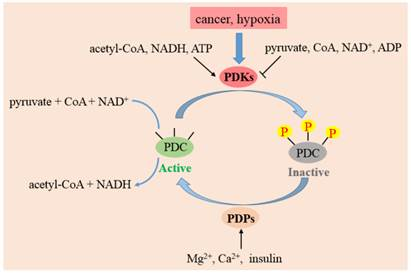
\includegraphics[width=0.45\textwidth]{TCA0_3}
	}
	\subfigure[regulation be products and educts]{
		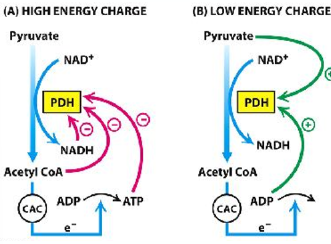
\includegraphics[width=0.45\textwidth]{TCA0_4}
	}
	\caption{Regulation of PDC/PDH}
\end{figure}

\subsubsection{TCA cylce steps}
The TCA cylce is a game of decarboxylation, generating energy by reduction of electron carriers. The formula: 
\begin{itemize}
	\item \textbf{Acteyl-CoA + GDP + Pi + 3 NAD+ + FAD => 2 CO2 + 3 NADH + FADH2 + GTP + CoA-SH}
\end{itemize}
\noindent \textit{In the bigger picture, this is were the CO2 is produced that we breathe out.}
\begin{figure}[H]
	\centering
	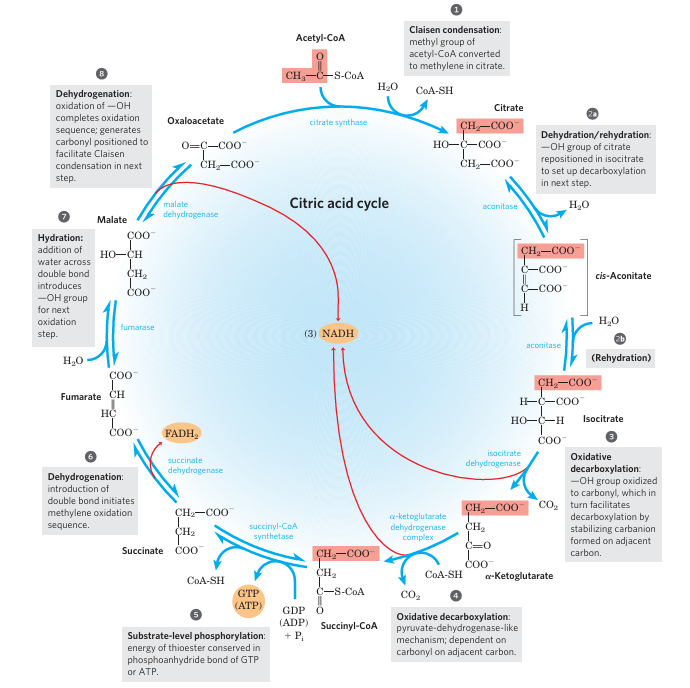
\includegraphics[width = \textwidth]{TCA1}
	\caption{Overview of the TCA cycle: The carbons shaded in red are those derived from the acetate of acteyl-CoA in the first turn.}
\end{figure}

\begin{RemarkWithTitel}{What happens to 3-14C-pyruvate}
	 The Resulting Acetyl-CoA will be labled at C2 (methyl group). Therfore, at the end of the first cycle: Oxaloacetate will be labelled in C2 or C3 (because of symmetry in succinate). After two more cycles, half of the label will be released. (the label of C2 ends up at the second cycle at C2 or C3, while the lable on C3 ends up at C4, which is released in the following clycle) But il will take an infinite number of cycles to release all the label. 
\end{RemarkWithTitel}


\paragraph{Step1: Formation of Citrate}
In the first step \textbf{the acetyl group} is transferred to \textbf{oxalacetate} to produce citrate. The reaction consists of two phases: (1) oxalycetate is condensed to acetyl-CoA to form citryl-CoA; (2) citryl-CoA is hydrolyzed to form citrate and CoA-SH. Whereby \textbf{phase 2 is highly exergonic} and therefore drives the entire reaction. 

\begin{RemarkWithTitel}{Citrate synthase}
	Step 1 is carried out by citrate synthase. Citrate synthase is a \textbf{dimer}. It first binds oxalacetate into its active site, which causes a conformational change from open to closed conformation. By doing so oxalacetate binding induces the formation of the acetyl-CoA binding site and shifts the catalytic residue into proper position. 
\end{RemarkWithTitel}

\begin{figure}[H]
	\centering
	\subfigure[reaction]{
		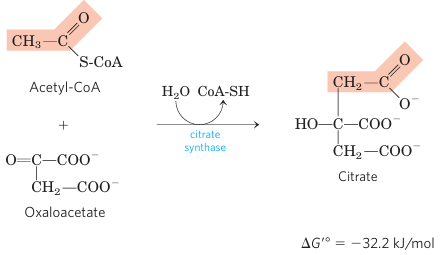
\includegraphics[width=0.45\textwidth]{TCAS1_1}
	}
	\subfigure[Citrate synthase]{
		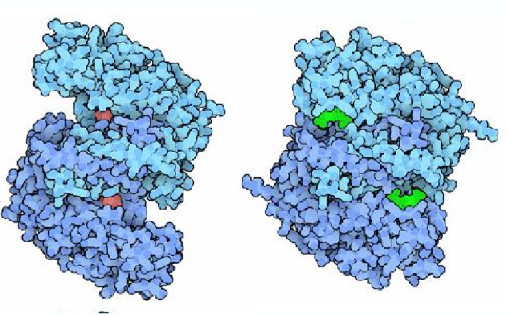
\includegraphics[width=0.45\textwidth]{TCAS1_2}
	}
	\caption{Formation of Citrate}
\end{figure}

\paragraph{Step2: Formation of Isocitrate}
Citrate is converted into isocitrate. In this reaction an hydroxyl group is moved from the third carbon of citrate to an adjacent carbon via a dehydration/hydration reaction. 

\begin{RemarkWithTitel}{Aconitase enzyme}
	Aconitase enzyme catalyzed this dehydration/hydration reaction. It contains a \textbf{Iron-Sulfur center}. 3 Cys residues of the enzyme bind 3 Fe atoms, the 4th is bound to one of the carboxyl groups of citrate and (non covalently) with a citrate hydroxyl group. \textbf{The Iron-Sulfur center acts in both substrate binding and catalysis}. 
\end{RemarkWithTitel}

\begin{figure}[H]
	\centering
	\subfigure[Creation of Isocitrate]{
		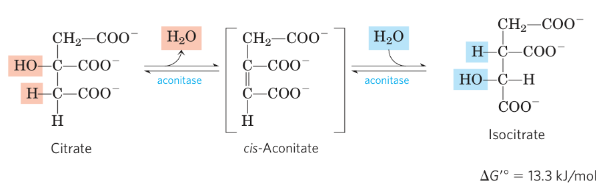
\includegraphics[width=0.55\textwidth]{TCAS2_1}
	}
	\subfigure[Aconitase enzyme]{
		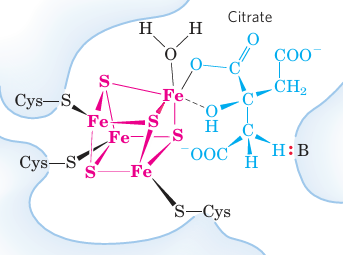
\includegraphics[width=0.4\textwidth]{TCAS2_2}
	}
	\caption{Formation of Isocitrate via cis-Aconitate}
\end{figure}

\paragraph{Step3: Decarboxylation of Isocitrate}
Once isocitrate is formed, it is ready to undergo the \textbf{first oxidative decarboxylation reaction} of the citric acid cycle. This step is catalyzed by \textbf{isocitrate dehydrogenase} which yields $\alpha$-ketoglutarate, CO2 and NADH

\begin{figure}[H]
	\centering
	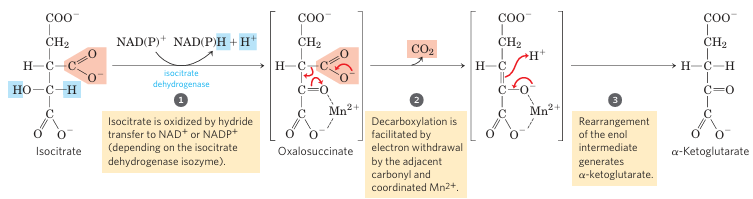
\includegraphics[width = \textwidth]{TCAS3}
	\caption{formation of $\alpha$-ketoglutarate by isocitrate dehydrogenase}
\end{figure}

\paragraph{Step4 Decarboxylation of $\alpha$-ketoglutarate}
This is the \textbf{second oxidative decarboxylation reaction} in the TCA cylce. $\alpha$-ketoglutarate is converted to succinyl-CoA with concomitant (at same time) production of \textbf{CO2 and NADH}. \textit{Note that the energy of the oxydation is conserved in the thiolester bond.}

\begin{RemarkWithTitel}{$\alpha$-ketoglutarte dehydrogenase complex}
	$\alpha$-ketoglutarte dehydrogenase complex is build very similar to the pyruvate dehydrogenase complex. Like PDC it has 3 has 3 importand enzymes: 
	\begin{itemize}
		\item E1: $\alpha$-ketoglutarate dehydrogenase with TPP as a cofactor
		\item E2: dihydrolipyl succiniltransferase with lipoic acid as a cofactor
		\item E3: dihydrolipyl dehydrogenase with FAD as cofactor. 
	\end{itemize}
	\noindent This is a clear case of \textbf{divergent evolution}. 
\end{RemarkWithTitel}

\begin{figure}[H]
	\centering
	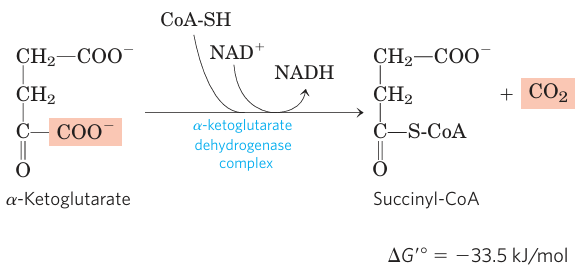
\includegraphics[height = 4 cm]{TCAS4}
	\caption{oxidation of $\alpha$-Ketoglutarate to Succinyl-CoA and CO2}
\end{figure}

\paragraph{Step5: Conversion of Succinyl-CoA to Succinate}
The unstable and high energy thiolester bond of succinyl-CoA is cleaved to release the CoA-SH unit. This releases free energy that is used used to produce GTP from GDP. This reaction is catalyzed by \textbf{succinyl CoA synthetases}. \\
The reaction has 3 phases as illustrated by fig. \ref{TCAS5_2}:
\begin{enumerate}
	\item A phosphate group substitutes CoA to form succinyl phosphate (a high energy acyl phosphate).
	\item Succinyl phosphate  donates the phosphate to a His residue in the enzyme (Succinat is formed).
	\item The phosphate group is transferred from the high energy phopsphorylated histidine to \textbf{GDP to form GTP}. 
\end{enumerate}
\begin{figure}[H]
	\centering
	\subfigure[Creation of Isocitrate]{
		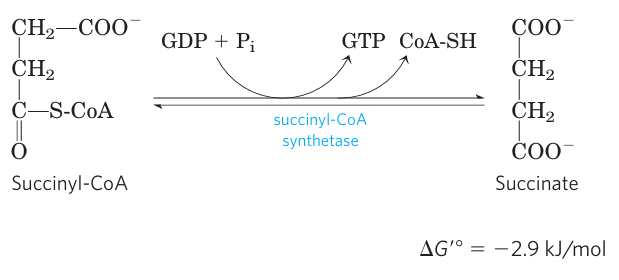
\includegraphics[width=0.5\textwidth]{TCAS5_1}
	}
	\subfigure[Aconitase enzyme]{
		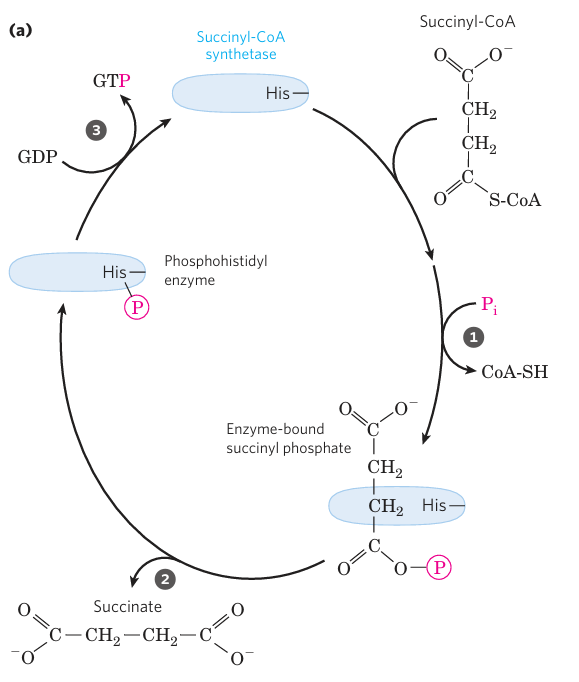
\includegraphics[width=0.45\textwidth]{TCAS5_2}
		\label{TCAS5_2}
	}
	\caption{Conversion of Succinyl-CoA to Succinate}
\end{figure}

\paragraph{Step6: Formation of Fumerate}
In step 6, succinate is oxidised to fumerate by succinate dehydrogenase. This is coupled to the reduction of FAD to FADH2. See fig. \ref{TCAS6}

\begin{RemarkWithTitel}{\gls{succinatedehydrogenase}}
	Succinate dehydrogenase is bound to the inner mitochondrial membrane and its FADH2 passes electrons to the electron transport chain. 
\end{RemarkWithTitel}


\paragraph{Step7: Formation of Malate}

\textbf{Fumerase} catalyses the hydration of fumerate into malate. Note that the water molecule attacks only at a specific site, thus only the \textbf{L}-isomer of malate is formed.

\begin{figure}[H]
	\centering
	\subfigure[Oxidation of Succinate to Fumerate]{
		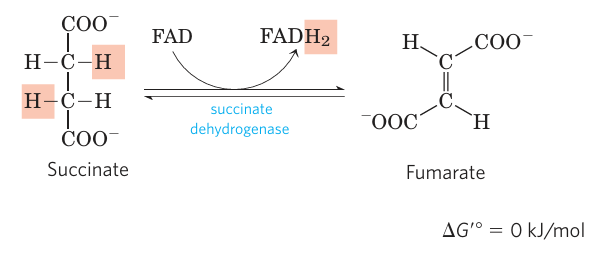
\includegraphics[width=0.45\textwidth]{TCAS6}
		\label{TCAS6}
	}
	\subfigure[Hydration of Fumerate into Malate]{
		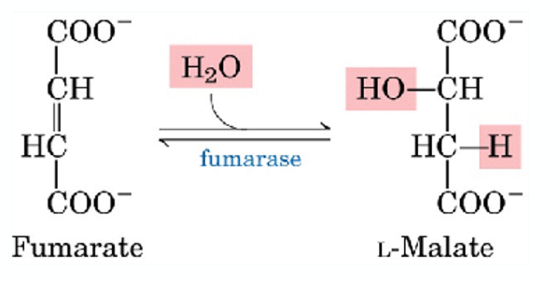
\includegraphics[width=0.45\textwidth]{TCAS7}
	}
	\caption{Step 6 and 7}
\end{figure}


\paragraph{Step8: Regeneration of Oxaloacetate}
Finally, \textbf{malate dehydrogenase} regenerates oxaloacetate by oxidation of malate. This reaction is couplet with the reduction of NAD+ to NADH. This process is highly \textbf{endergonic} and needs to be coupled with other exergonic steps.  

\begin{figure}[H]
	\centering
	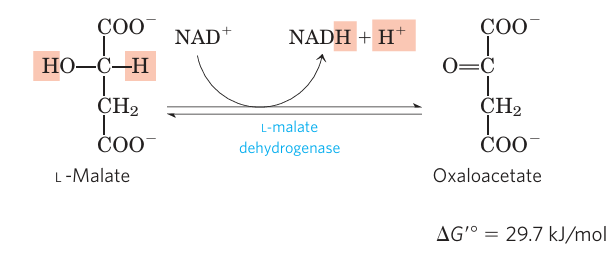
\includegraphics[height = 4 cm]{TCAS8}
	\caption{Oxidation of Malate to Oxaloacetate}
\end{figure}


\subsection{Fatty Acid Oxidation}
Adipose tissue cells (\textbf{adipocytes}) are specialised cells that store energy in the form of \textbf{triglycerides}. \textit{Lipids are a form to long-time store energy, which will be used in moments with little glucose.} Upon demand triglycerides are hydrolysed to glycerol and fatty acids that are transported to target tissues. \\
Following this step \textbf{fatty acids} can be \textbf{activated (bound to CoA, see. fig. \ref{FA0_4})} and transported to the mitochondrial matrix of cells. In the mitochondrial matrix they iteratively undergo a series of \textbf{4 reactions} that shorten the acyl chain by 2 carbons and release acetyl-CoA (that can feed in the TCA cycle)\\
This entire process is known as \textbf{fatty acid oxidation}. \\
\\
Dietary fats are absorbed in the \textbf{small intestine}. \textbf{\gls{bileacids}} are released an act as biological detergents, resuspending tryglcerides into fine micelles. In this form triglycerides are accessible to water-soluble lipases in the intestine lumen. \\
The products of this lipasen are then absorbed by the intestine mucosa and converted back to triglycerides. They are then transported through the bloodstream and finally stored in dedicated adipose cells that have the specialized organelles named \textbf{lipid droplets}.

\begin{RemarkWithTitel}{Triacylglcerols better then Polysaccharides}
	Triacylglcerols contain \textbf{more energy per gram then polysaccharides}. Moreover, the are unhydrated, thus the oranism does not have to carry the extra weight in form of water as with stored polysaccharides. Additionally in some animals, such as seals, fats stores under the skin serve as insulation against cold temperatures. 
\end{RemarkWithTitel}
\begin{figure}[H]
	\centering
	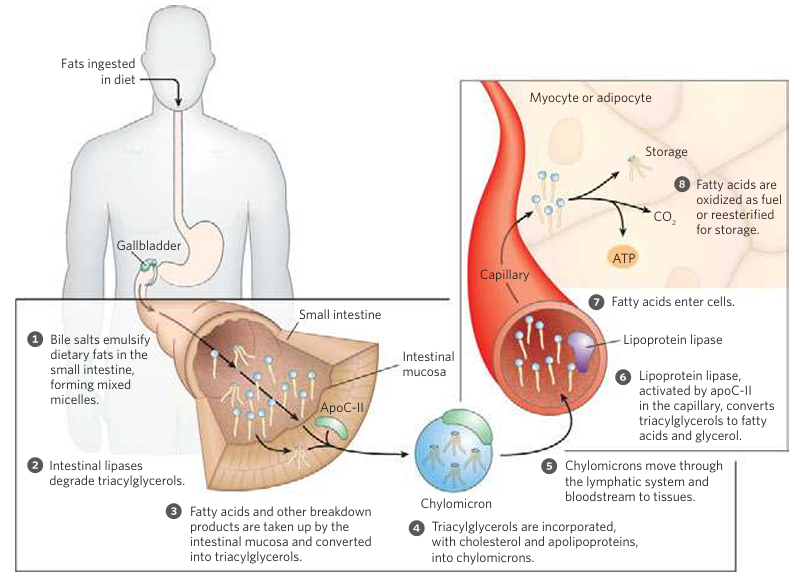
\includegraphics[width = 0.8 \textwidth]{FA0_2}
	\caption{Processing of dietary lipids in vertebrates}
\end{figure}
\noindent
When blood glucose levels are low, some hormones (\textbf{glucagon/adrenaline}) are released. They activated \textbf{adenylyl cyclase on the surface of adipocites}. This leads to the production of \textbf{cAMP} which activats \textbf{protein kinase A (PKA)}, which triggers intracellular triglyceride lipase to produce fatty acids and glycerol. The products are released into the bloodstream, where they are transported with the serum protein \textbf{Albumin} to muscle cells (\textbf{mycocytes}) where they are then oxidized for the production of ATP. 

\begin{figure}[H]
	\centering
	\subfigure[Mobilization of tracylglycerols stored in adipose tissue]{
		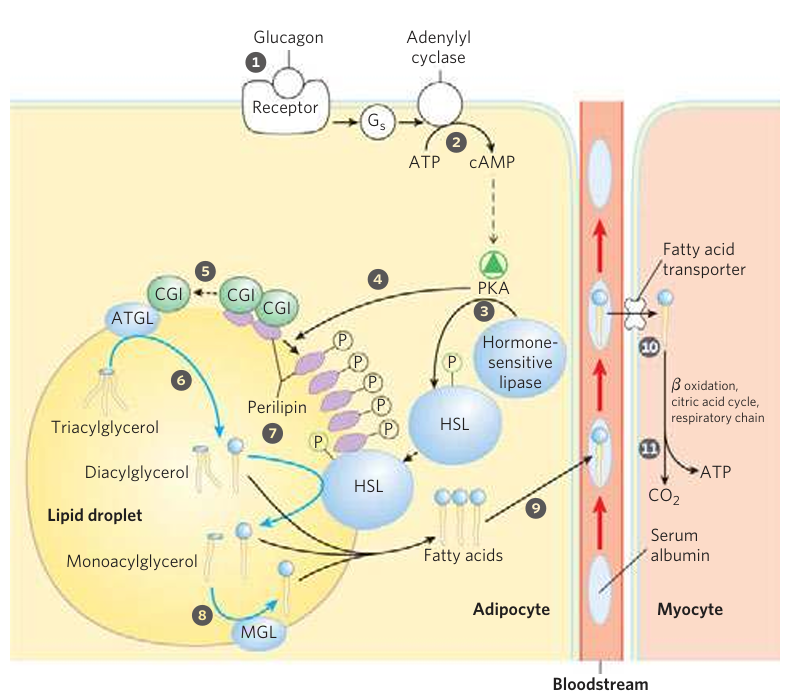
\includegraphics[height = 8cm]{FA0_1}
	}
	\hfil
	\subfigure[Adipose tissue]{
		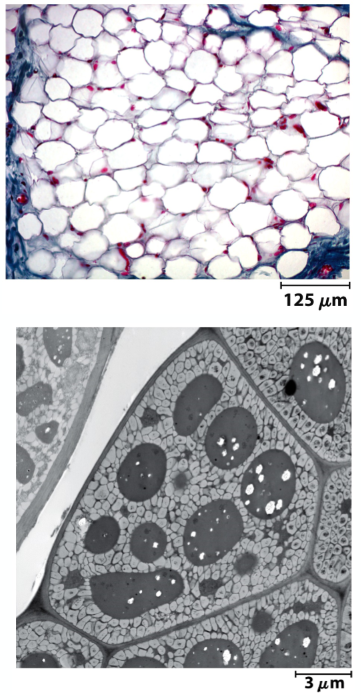
\includegraphics[height = 8 cm]{FA0_3}
	}
	\caption{}
\end{figure}
 
\paragraph{What about glycerol?}
95\% of the energy derived from triglycerides comes from the oxidation of the fatty acid chain, where only \textbf{5\% comes from glycerol}.\\
\indent Glycerol, released by triglyceride lipases, is phosphorylated to glycerol 3-phopsphate by \textbf{glycerol kinase} using 1 ATP. Then glycerol is oxidized by the enzyme glycerol 3-phosphate dehydrogenase to \textbf{DHAP}, thus entering the glycolytic pathway. 

\begin{RemarkWithTitel}{How much ATP do we get from glycerol in the glycolytic pathway?}
	First we have to invest 1 ATP to produce DHAP entering the glycolytic pathway. We enter the payoff phase of glycolysis where we produce 2 ATP. Giving us a net of 1 ATP produced, additionally we still have the energy of 1 pyruvate and 2 NADH. 
\end{RemarkWithTitel}

\paragraph{Transport into the Mitochondria}
\textbf{The transport into the mitochondria is the rate-limiting step in $\beta$-oxidation}.\\
Fatty acid oxidation takes place in the mitochondrial matrix. Therefore fatty acids have to be transported into the mitochondria to be oxidized. For this purpose, they are again activated, linked to CoA. This is done by the enzyme \textbf{fatty acyl-CoA synthetases}\\
\\
Fatty acyl-CoA synthetases have a \textbf{two phase mechanism} (see fig. \ref{FA0_4}): 
\begin{enumerate}
	\item The fatty acid made reactive by forming a complex with AMP, producing PPi and using ATP. 
	\item AMP is then exchanged with CoA-SH, in a nucleophilc attack, forming fatty acyl-CoA. 
\end{enumerate}
\noindent \textit{Note that PPi is immediately dissociated into phosphate molecules by inorganic pyrophosphatase. } 

\begin{figure}[H]
	\centering
	\subfigure[Conversion of a fatty acid to fatty acyl-CoA]{
		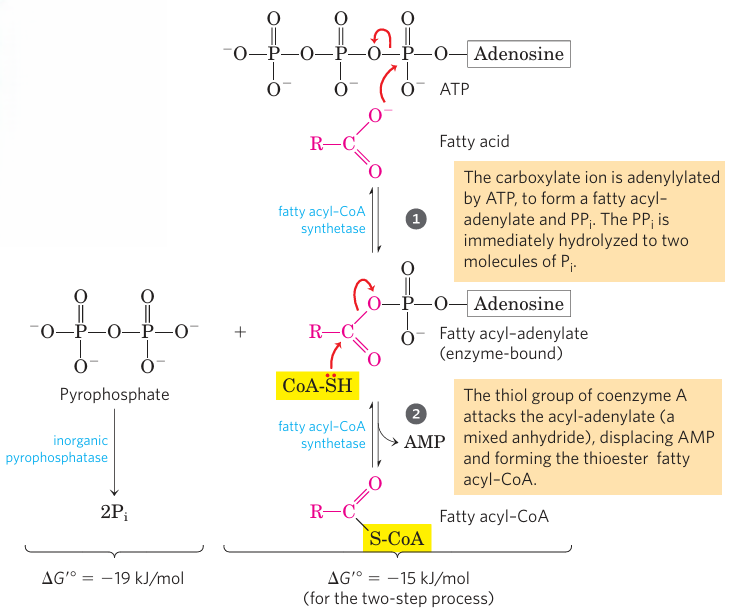
\includegraphics[height = 8cm]{FA0_4}
		\label{FA0_4}
	}
	\hfil
	\subfigure[Formula of L-Carnitine]{
		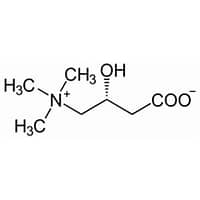
\includegraphics[height = 4 cm]{carnitine}
		\label{carnitine}
	}
	\caption{}
\end{figure}
\noindent
Once formed in the cytosolic environment, fatty acyl-CoA crosses the mitochondrial membrane transiently exchanging its CoA with carnitine and exploiting the \textbf{acyl-carnitine transporter}.
\begin{itemize}
	\item Carnitine acyltransferase \textbf{I} is located at the outer membrane and catalyzes the exchange of CoA with carnitine. 
	\item Carnitine acyltransferase \textbf{II} is located in the inner membrane and exchanges the carnitine for CoA. 
\end{itemize}
		
\begin{DefWithTitle}{Carnitine}
	\gls{carnitine} (see. fig \ref{carnitine}) is a quaternary ammonium compound. Carnitine forms a temporary conjugate with acyl groups (as acyl-carnitine), enabling them to cross the inner mitochondrial membrane via the carnitine shuttle system.
\end{DefWithTitle}

\begin{figure}[H]
	\centering
	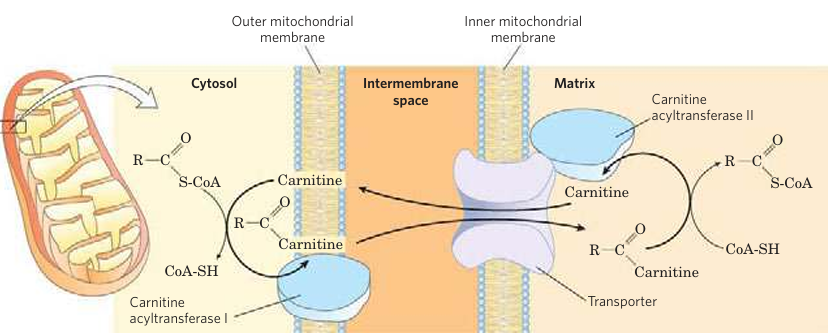
\includegraphics[width = 0.8 \textwidth]{FA0_5}
	\caption{Fatty acid entry into mitochondria via acyl-carnitine/carnitine transporter}
\end{figure}

 \begin{RemarkWithTitel}{Primary Carnitine deficiency}
	Primary carnitine deficiency is an autosomal recessive disorder affecting transport of carnitine. Since carnitine is essential for the transport of long-chain fatty acyl-CoA into the mitochondria, this disorder results in reduced fatty acid-derived energy production, leading to symptoms such as \textbf{fatigue}. Moreover, impaired import of fatty acids into mitochondria causes their accumulation in the cytoplasm (\textbf{lipotoxity}), which can disrupt organ function. In the heart, this may result in cardiomyopathy.
\end{RemarkWithTitel}


\subsubsection{Beta oxidation}
There are 3 stages in the oxidation of FAs (see fig. \ref{FA1_1}). The \textbf{$\beta$-oxidation} is the first stage, where, in the mitochondrial matrix, fatty acetyl-CoA is progressively oxidised by an \textbf{iterative sequence of four reactions that produce acetyl-CoA} \\
\indent The acetyl-CoA units formed in stage 1 can then be feed in the TCA cycle (stage 2). Finally, the electrons subtracted in these oxidative reactions are used to produce ATP in the ETC. \\
\\
There are 4 reactions involved in $\beta$-oxidation (see fig. \ref{FA1_2}): 
\begin{enumerate}
	\item Dehydrogenation produces a double bond between the $\alpha$- and $\beta$-carbon (C2 and C3). This is catalyzed by \textbf{acyl-CoA dehydrogenase} (similar to succinate dehydrogenase from TCA cycle) and produces \textbf{1 FADH2}.
	\item Hydration, adding water to the $\alpha$-$\beta$ double bond. The hydroxy group is added to C3, producing $\beta$-Hydroxyacyl-CoA. This is done by \textbf{enoyl-CoA hydratase}
	\item Dehydrogenation, oxidizing the alcohol group to a keton, produces $\beta$-Ketoacyl-CoA. This is done by \textbf{$\beta$-hydroxyacyl-CoA dehydrogenase}, whose action is homologous to that of malate dehydrogenase in the TCA cycle. The electrons are transferred to NAD+ creating \textbf{NADH}
	\item Finally the chain is shortened by a thiolase which \textbf{detaches Acetyl-CoA} and creates a by 2 carbon shorter Acyl-CoA. This is catalyzed by \textbf{acyl-CoA acetyl transferase}. 
\end{enumerate}

\begin{figure}[H]
	\centering
	\subfigure[Stages of FA oxidation]{
		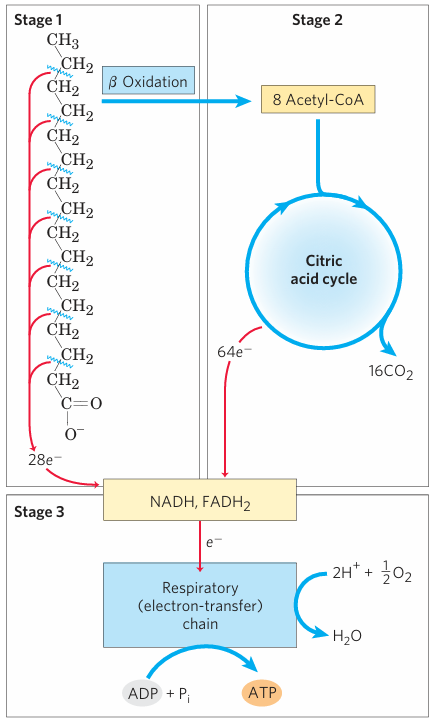
\includegraphics[width = 0.45 \textwidth]{FA1_1}
		\label{FA1_1}
	}
	\hfil
	\subfigure[$\beta$-oxidation pathway]{
		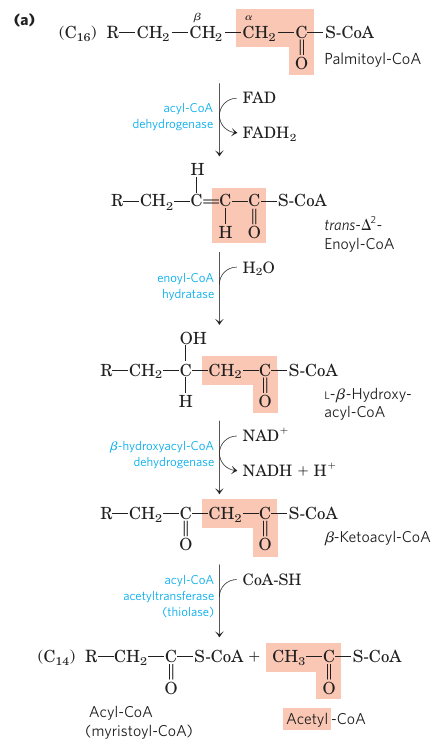
\includegraphics[width = 0.45 \textwidth]{FA1_2}
		\label{FA1_2}
	}
	\caption{FA oxidation overview}
\end{figure}

\begin{RemarkWithTitel}{Unsaturated FAs}
 	In the case of unsaturated fatty acids, two more enzymes are required (see fig. \ref{FA1_3}): 
 	\begin{itemize}
 		\item \textbf{Enoyl-CoA isomerase} that converts the \textbf{cis-isomer into a trans-isomer} or/and \textbf{shift the double bond} to the right position (C2=C3), which can be used by enoyl hydratase. (Obviously only for FA containg cis double bounds)
 		\item For \textbf{polyunsaturated FAs} \textbf{(2) 2,4-dienoyl-CoA reductase} has to be used. It reduces 2 double bounds to one, \textbf{consuming an NAD\underline{P}H}. Following this step, the \textbf{enoyl-CoA isomerase} can act on the substrate and make it degradable by $\beta$-oxidation.
 	\end{itemize}

\end{RemarkWithTitel}

\begin{RemarkWithTitel}{Odd-number FAs}
	Although the vast majority of FA are constituted by an even number of carbons. Odd-number FAs exist and need to be degraded in the same way, but at the \textbf{last iteration} of $\beta$-oxidation, they yield \textbf{propionyl-CoA} instead of acetyl-CoA.\\
	\\
	The enzyme \textbf{propionyl-CoA carboxylase} is used to produce D-methylmalonyl-CoA, which can be converted through two further ractions to succinyl-CoA. \textbf{Succinyl-CoA} can then enter the TCA cycle. See fig. \ref{FA1_4}

\end{RemarkWithTitel}

\begin{figure}[H]
	\centering
	\subfigure[Oxidation of \textbf{polyunsaturated} fatty acid]{
		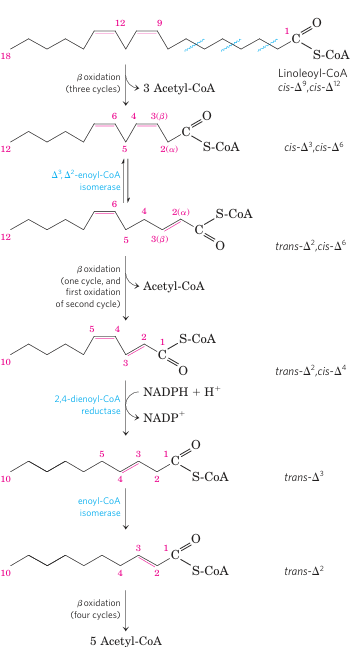
\includegraphics[width = 0.45 \textwidth]{FA1_3}
		\label{FA1_3}
	}
	\hfil
	\subfigure[Oxidation of \textbf{odd-number} fatty acids]{
		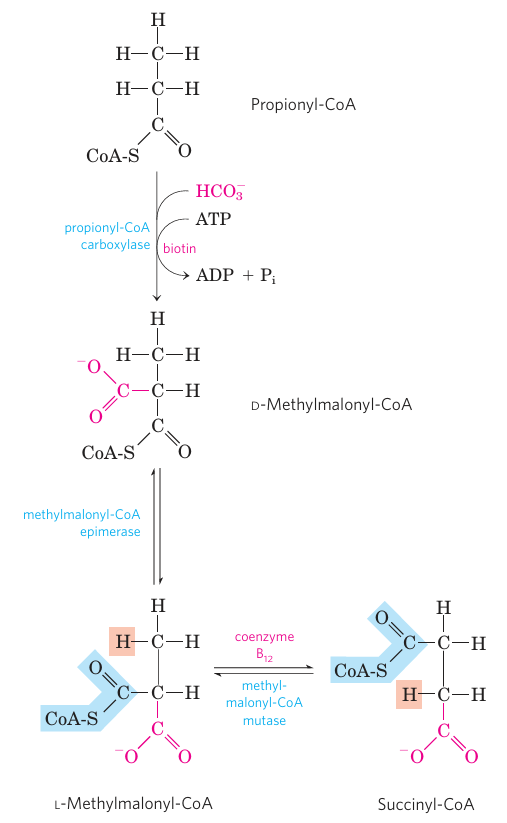
\includegraphics[width = 0.45 \textwidth]{FA1_4}
		\label{FA1_4}
	}
	\caption{FA oxidation overview}
\end{figure}

\paragraph{Calculate amount of ATP from a FA of given length}
\textit{This section assumes the fucked up numbers given in ETC for NADH and FADH2, sucks!}\\
\\
\noindent
\underline{Assuming the FA is fully saturated and consists of \( n \) carbons (even number):}\\
\\
\textbf{Number of $\beta$-oxidation cycles:}
\[
\frac{n}{2} - 1
\]
\textbf{Each $\beta$-oxidation cycle produces:}
\begin{itemize}
	\item 1 NADH $\rightarrow$ 3 ATP
	\item 1 FADH\textsubscript{2} $\rightarrow$ 2 ATP
	\item 1 Acetyl-CoA (last cycle gives 2) $\rightarrow$ 12 ATP via TCA
\end{itemize}
\noindent
\textbf{Each acetyl-CoA entering the citric acid (TCA) cycle generates:}
\begin{itemize}
	\item 3 NADH $\rightarrow$ $3 \times 3 = 9$ ATP
	\item 1 FADH\textsubscript{2} $\rightarrow$ $1 \times 2 = 2$ ATP
	\item 1 GTP (equivalent to ATP) $\rightarrow$ $1$ ATP
\end{itemize}
\noindent
\textbf{Activation of FA to Co-A costs 2 ATP.}
\\
\textbf{Total ATP yield:}
\[
\text{ATP}_{\text{total}} = \left( \frac{n}{2} - 1 \right) \cdot (3 + 2) + \frac{n}{2} \cdot 12 - 2
\]
\noindent
\\
\underline{If we have an odd number of carbons:}\\
\\ 
\noindent
\textbf{Account for Propionyl-CoA $\rightarrow$ Succinyl-CoA:}
\begin{itemize}
	\item 1 NADH → 3 ATP
	\item 1 FADH\textsubscript{2} → 2 ATP
	\item 1 GTP → 1 ATP
\end{itemize}
\noindent
\[
\text{ATP}_{\text{total}} = \left\lfloor \frac{n}{2} \right\rfloor \cdot 5 + \left\lfloor \frac{n}{2} \right\rfloor \cdot 12 + 6 - 2
\]
\underline{ATP Yield from a Polyunsaturated Fatty Acid:}
\[
\text{ATP}_{\text{total}} = \left( \frac{n}{2} - 1 \right) \cdot 5 + \left( \frac{n}{2} \cdot 12 \right) - (p \cdot 2) - (q \cdot 3) - 2
\]
Where:
\begin{itemize}
	\item \( p \): Number of double bond "islands"; each skips FADH\textsubscript{2} production (–2 ATP).
	\item \( q \): Sum of (number of connected double bonds in one island – 1); each costs 1 NADPH (–3 ATP).
\end{itemize}


\subsection{Amino Acid Catabolism}
Amino acids that are derived from the degredation of proteins are the third class of biomolecules (after carbohydrates and fatty acids) that significantly contribute to the cellular energy metabolism. \\
\\
In animals amino acids are oxidised in three different mataboltic conditions: 
\begin{itemize}
	\item During protein turnover some amino acids can be oxidized, if they are not required for the synthesis of other proteins. 
	\item In a protein rich diet, food-derived amino acids can exceed the needs for protein biosynthesis. Note there is no way to store amino acids.
	\item In starvation when carbohydrates are not available. AA from endergenous (produced within the body) proteins are used as an energy source.   
\end{itemize}
Amino acids are split into a carbon skeleton and an amino group (which contains nitrogen). The carbon skeleton can be used for energy production or biosynthesis. The amino group, however, is converted into ammonia (NH3), which is toxic to our cells.
\begin{figure}[H]
	\centering
	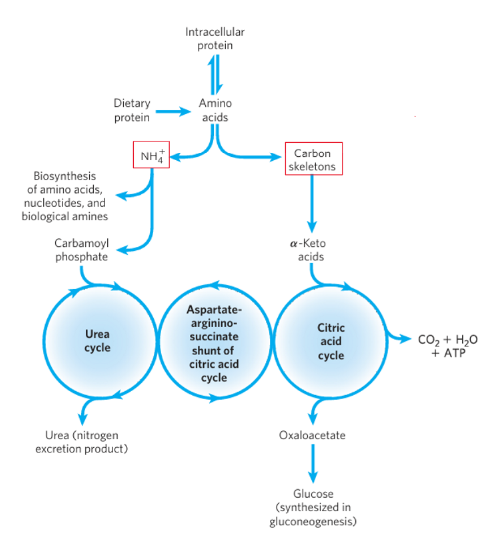
\includegraphics[width = 0.7 \textwidth]{AA1_1}
	\caption{Overviw of amino acid catabolism in mammals}
\end{figure}

\subsubsection{AA oxidation and Urea production}

The first step is the detachment of the $\alpha$ amino group. This is catalyzed by \textbf{amino transferase} that transfers the amino group to the $\alpha$-ketoglutarate to form a \textbf{$\alpha$-keto acid}. \\
\\
The amino tranferase requires the \textbf{cofactor \gls{plp}}, a derivative of Vitamine B6. PLP acts as a \textbf{transitory transporter of amino groups}. \\
\\
One formed in the cytoplasm, glutamate is transported in the mitochondria where it undergoes \textbf{oxidative deamination} catalyzed by \textbf{glutmamate dehydrogenase} that oxidizes glutamate back to $\alpha$-ketoglutarate and creats NH4+. This reaction is coupled to the reduction of NAD(P)+ to NAD(P)H. \\
\\
\textbf{Glutmamate dehydrogenase} is tighly controlled by the energy charge. GTP (indicating high energy charge) acts as an inhibitor and ADP (indicating low energy charge) acts as a simulator. 
 
\begin{figure}[H]
	\centering
	\subfigure[Enzyme-catalyzed transamination]{
		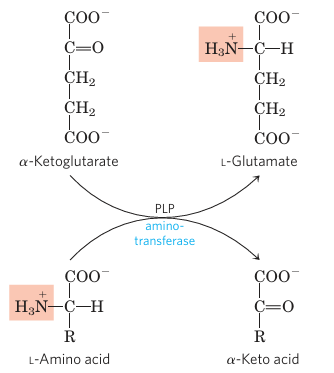
\includegraphics[width = 0.3 \textwidth]{AA2_1}
	}
	\subfigure[Cofactor PLP]{
		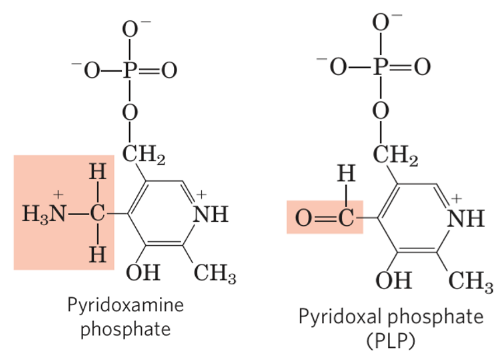
\includegraphics[width = 0.2 \textwidth]{AA2_2}
	}
		\subfigure[Regulation of glutamate dehydrogenase]{
		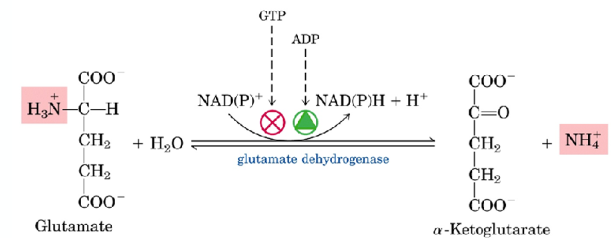
\includegraphics[width = 0.4 \textwidth]{AA2_5}
	}
	\caption{Amino acid oxidation and urea production}
\end{figure}

\begin{figure}[H]
	\centering
	\includegraphics[width = 0.8\textwidth]{AA1_2}
	\caption{Amino group catabolism}
	\label{AA1_2}
\end{figure}

\paragraph{Ammonia transport}
Ammonia is toxic for most tissues. Thus, in order to be transported to the liver where it is converted into urea, it needs to be incorporated into a non-toxic compound. \\
\indent In most tissues ammonia is therefore complexed to glutamate to produce glutamine. This is done by the enzyme \textbf{glutamine synthetase} and requires \textbf{ATP}. See fig. \ref{AA2_6} \\
\textit{Note this a perfect example how ATP hydrolysis can foster otherwise unfavorable reactions.}\\
\indent Once in the \textbf{liver's mitochondria this is reversed by glutaminase}. See fig. \ref{AA2_6}\\
\\ 
In the \textbf{muscle} and other tissues where amino acids are intensively used for the production of energy, the \textbf{amino group can be transferred to pyruvate} to form alanine. Which can be transported to the liver. See fig. \ref{AA2_3}

\begin{figure}[H]
	\centering
	\subfigure[Glutamine]{
		\includegraphics[width = 0.4 \textwidth]{AA2_6}
		\label{AA2_6}
	}
	\hfil
	\subfigure[Alanine]{
		\includegraphics[width = 0.5 \textwidth]{AA2_3}
		\label{AA2_3}
	}
	\caption{Transport of Ammonia}
\end{figure}

\paragraph{Urea production}
Once transported to liver mitochondria converted to urea in a serie of 4 reactions (\textbf{the Urea cycle}). The first happens in the mitochondrial matrix while the remaining three happen in the cytosol. 
\begin{enumerate}
	\item Citrulline is formed from Ornithine by the addition of a carbamoyl group. \textbf{Carbamoyl} carries the ammonia from glutamine. The construction of Carbomyl used 2 ATP.
	\item Argininosuccinate is formed by condensation of citrulline and asparate. This uses ATP.
	\item Argininosuccinate is decomposed in \textbf{fumarate} (that feeds in the TCA cylce) and arginine.
	\item Arginine is decomposed into urea and ornithine by \textbf{arginase}
\end{enumerate}
\paragraph{Entry in TCA}
As there are 20 amino acids there are 20 catablolic pathways for those amino acids. 
\begin{figure}[H]
	\centering
	\includegraphics[width = 0.7 \textwidth]{AA2_4}
	\caption{Glucose-alanine cylce}
\end{figure}  

\begin{RemarkWithTitel}{Deffects in amino acid matabolism}
	Several genetic defects have been identified in humans that impact the amino acid matabolism. These defects lead to the accumulation of neurotoxic intermeadiates resulting in intellectual disabilities. 
\end{RemarkWithTitel}


\subsection{Oxidative Phosphorylation}
The process of aerobic respiration is completed in the \textbf{mitochondria} by oxidative phosphorylation. The NADH molecules formed in glycolysis as well as the NADH and FADH2 molecules formed in TCA cycle, in $\beta$-oxidation and in the amino oxidation are used to produce ATP along the \textbf{electron transport chain (ETC)}.

\begin{itemize}
	\item A NADH molecule in the mitochondrial matrix yields 3 ATP. 
	\item A cytosolic NADH or FADH2 yields 2 ATP
\end{itemize}

\subsubsection{ECT}
The electron transport chain (ETC) is a series of protein complexes that reside in the \textbf{inner mitochondrial membrane}. The ETC transports electrons, creating an electrical current that is coupled to the \textbf{pumping of H+ ions from the mitochondrial matrix to the inter-membrane mitochondrial space}. \\
Note: 
\begin{itemize}
	\item The outer mitochondrial membrane is permeable to the majority of small molecules and anions (\textbf{not} cations [H+]) due to the presence of mitochondrial porins.
	\item The inner mitochondrial membrane lacks porins and is thus impermeable to ions and small metabolites that require specialised transporters to leave the mitochondrial matrix. 
\end{itemize}
\noindent 
The ETC consists of 4 protein complexes that accept the electrons from NADH and FADH2 and move the electrons along the inner mitochondrial membrane onto \textbf{the finally acceptor oxygen}. This produces the protein gradient which is exploited by ATP synthase to produce ATP.

\begin{figure}[H]
	\centering
	\includegraphics[width = 0.8 \textwidth]{ETC0}
	\label{ETC0}
	\caption{Overview of the ETC}
\end{figure}  

\begin{RemarkWithTitel}{Coenzyme Q}
	\gls{ubiquinone}, is a \textbf{hydrophobic electron carrier} that can dissolve in the inner mitochondrial membrane bilayer. It can accepts 1 or 2 electrons thus being reduced to Semiquinone ($\boldsymbol{\cdot}$QH) and Ubiquinol (QH2) respectively. See fig. \ref{ETC2}\\
	It serves a sa transporter from \textbf{Complex I to II and II to III}. 
\end{RemarkWithTitel}

\begin{RemarkWithTitel}{Cytochrome C}
	A small \textbf{heme protein} located in the intermembrane space of mitochondria. See fig. \ref{ETC3} \\
	\\
	Cytochrome C is highly \textbf{water-soluble}, and is able to undergo \textbf{oxidation and reduction} as its iron atom converts between the ferrous(2+) and ferric(3+) forms. (it does \textit{not} bind oxygen)\\
	\\
	It plays a key role in the electron transport chain by transferring electrons between \textbf{Complex III} (cytochrome bc\textsubscript{1} complex) and \textbf{Complex IV} (cytochrome c oxidase)
\end{RemarkWithTitel}

\begin{figure}[H]
	\centering
	\subfigure[Coenzyme Q]{
		\includegraphics[height = 6 cm ]{ETC2}
		\label{ETC2}
	}
	\hfil
	\subfigure[Cytochrome C]{
		\includegraphics[height = 6 cm]{ETC3}
		\label{ETC3}
	}
	\caption{Electron carrier in the ETC}
\end{figure}


\begin{DefWithTitle}{Fe-S clusters}
	Iron-sulfur clusters occur in many biological systems, often as components of \textbf{electron transfer proteins}. The relevant redox couple in all Fe-S proteins is\textbf{ Fe(II)/Fe(III)}. \\
	They may be more or less complex (see. fig. \ref{ETC1})
\end{DefWithTitle}

\begin{figure}[H]
	\centering
	\includegraphics[width = 0.7 \textwidth]{ETC1}
	\label{ETC1}
	\caption{Iron-sulfur centers}
\end{figure}

\paragraph{Complex 1}
Complex I (NADH dehydrogenase or NADH oxidoreductase), is a very lagre protein complex consisting of 46 polypeptides. It has a L shape. One arm  lies withing the inner membrane while the vertical component lies in the matrix. \\
\\
Complex I receives high energy electrons from \textbf{NADH}. NADH donates electrons to a series to FMN, leading to the reduction of FMN to \textbf{FMNH2}. FMNH2 then donates the electrons to a s\textbf{eries of Fe-S clusters}. Finally two alectrons are transferred to CoQ producing \textbf{CoQH2}. See fig. \ref{ETCC1}\\
\\
As the electrons move along the series of Fe-S clusters, the complex uses the electrical power t pump a total of \textbf{4H+} into the intermembrane space. 

\begin{figure}[H]
	\centering
	\subfigure[NADH:ubiquinone oxidoreductase (Complex I)]{
		\includegraphics[width = 0.5 \textwidth]{ETCC1}
		\label{ETCC1}
	}
	\subfigure[Potentials]{
		\includegraphics[width = 0.45 \textwidth]{ETCC1_1}
		\label{ETCC1_1}
	}
	\caption{}
\end{figure}


\paragraph{Complex 2}
\textbf{Complex II is the succinate dehydrogenase used in to TCA cycle} to form fumerate from succinate (\textbf{step 6}). Note complex II is \textbf{not} a proton pump. \\
\\
The \textbf{FADH2} is created in step 6 of the TCA cycle and stays tightly connected to the enzyme. FADH2 transferres his \textbf{2 high energy electrons} to a series of \textbf{Fe-S clusters} that ultimately transfer the electrons to CoQ producing \textbf{CoQH2}. See fig. \ref{ETCC2}.\\
\textit{Note, Hemme b group does not appear to be part of the electron thransporting pathway. }

\begin{figure}[H]
	\centering
	\includegraphics[width = 0.5 \textwidth]{ETCC2}
	\caption{Complex II - succinate dehydrogenase}
	\label{ETCC2}
\end{figure}

\paragraph{Complex 3}
Complex III \textbf{transfers electrons from CoQH2 to Cytochrome c}. This is done through the Q cycle, which has two stages: 
\begin{enumerate}
	\item In the first half cycle \textbf{CoQH2} binds to the complex III and transfers \textbf{one electron} to the \textbf{Rieske center}. From there it is transferred to \textbf{Cyt c1} and then to \textbf{Cyt c}. This reaction \textbf{pumps 2 H+}.\\
	The \textbf{second electron} is transferred from \textbf{Cyt b} to an other CoQ producing \textbf{*CoQH}.
	\item In the second half cycle is practically a repetition of the first, but the \textbf{second electron is transferred to the *CoQH} produced in the first half cycle. The resulting QH2 is released back into the Q pool. 
\end{enumerate}
\noindent
This leads to the net equation of: \textbf{QH2 + 2 cyt c1 (oxidized) + 2H+ => Q + 2 cyt c1 (reduced) + 4H+}. Therefore \textbf{pumping 4H+} andt the reduced cyt c is transferred to the complex IV. 

\begin{figure}[H]
	\centering
	\subfigure[Complex III - cytochrome $bc_{1}$]{
		\includegraphics[width = 0.5\textwidth]{ETCC3}
		\label{ETCC3}
	}
	\hfil
	\subfigure[The Q cycle]{
		\includegraphics[width = 0.4\textwidth]{ETCC3_1}
		\label{ETCC3_1}
	}
	\caption{Complex III}
\end{figure}

\paragraph{Complex 4}
Complex IV transfers the electrons received form complex III via \textbf{cytochrome c to oxygen}. Complex IV pumps 4H+ using 4 Cyt c. This happens in 4 steps: 
\begin{enumerate}
	\item Two reduced Cyt c give off 2 electrons. One goes to Hemme $a_{3}$ and the other to $Cu_{B}$
	\item once Hemme $a_{3}$ and $Cu_{B}$ are reduced , 1 O2 molecule can bind and abstract 2 electrons thus forming a peroxide bridge.
	\item Two additional Cyt c are reduced transferring their electrons to 2H+ (from the matrix). They then break the peroxide bridege and forme Hemme $a_{3}$-OH and $Cu_{B}$-OH
	\item Two additional protons from the matrix oxidize Hemme $a_{3}$ and $Cu_{B}$ to their original state producing 2 molecules of water. 
\end{enumerate}
\noindent This \textbf{pumps 4H+} in the intermembrane space. Sometimes also referred as 2H+, in this case it used 2 Cyt and 0.5 O2. 

\begin{figure}[H]
	\centering
	\subfigure[Complex IV - cytochrome oxidase]{
		\includegraphics[width = 0.5 \textwidth]{ETCC4}
		\label{ETCC4}
	}
	\subfigure[Reactive Oxygen Species]{
		\includegraphics[width = 0.45\textwidth]{ECTROS}
		\label{ETCROS}
	}
	\caption{Complex IV and ROS}
\end{figure}


\begin{RemarkWithTitel}{Reactive Oxygen Species (ROS)}
	ROS are chemically reactive species containing oxygen. ROS are produced in a variety of biochemical reactions / organelles such as peroxisomes, \textbf{mitochondria}, etc. . \\
	In the ETC about 0.1-2\% of electrons are \textbf{prematurely transferred to oxygen}. Specific enzymes in our mitochondrias are used to detoxify \textbf{superoxyde radicals}, be converting them to \textbf{hydrogen peroxide} and then to \textbf{water}. See fig. \ref{ETCROS} 
\end{RemarkWithTitel}

\subsubsection{ATP synthase - Complex V}
The ATP synthase generates ATP molecules using the proton motive force due to the H+ gradient to release ATP into the mitochondria. \\
The structure consists of two major regions, F0 and F1: 
\begin{itemize}
	\item \textbf{F0} is \textbf{hydrophobic} and lies within the inner membrane. It consists of \textbf{10-14 c subunits} organised in a ring; a single \textbf{a subunit} and \textbf{2 b subunits}.  
	\item \textbf{F1} is the \textbf{catalytic region}. It lies in the matrix of the mitochondria and it is consituded by five polypeptides: \textbf{3 alpha}, \textbf{3 beta}, \textbf{gamma}, \textbf{delta}, and \textbf{epsilon}. 
\end{itemize}
\noindent Each unit has its purpose: 
\begin{itemize}
	\item The \textbf{alpha and beta} subunits form an \textbf{hexametrix hetero-oligome}r having a central cavity.
	\item The \textbf{gamma and epsilon} subinits form what is called  the \textbf{central stalk} that runs through the cavity of the beta/alpha hexamer.
	\item The \textbf{delta} subunit keeps the alpha/beta hexamer from rotating.
	\item The \textbf{c ring} and the \textbf{a subunit} works as a proton channel. The c ring also rotates because of the proton flow. This also rotates the  central stalk. 
\end{itemize} 
\noindent \textit{Note that the a, b , delta, alpha, and beta subints do not rotated.} \\
\\
\begin{figure}[H]
	\centering
	\includegraphics[width = 0.5 \textwidth]{ATPS1}
	\caption{ATP synthase}
	\label{ATPS1}
\end{figure}
\noindent Note in figure \ref{ATPS2} N side = matrix and P side = intermembrane space. 

\begin{RemarkWithTitel}{Why does C rotate?}
	First note that the a subunit spans the entire membrane. So first an \textbf{H+ enters the a subunit} from the matrix and binds to the \textbf{asparate residue in the closest c subunit}. Through the pressure of more H+ comming into the a subint the \textbf{c ring turns} until the H+ finds the \textbf{exit in other half of the a subint}. See fig. \ref{ATPS3}
\end{RemarkWithTitel}

\begin{RemarkWithTitel}{How does the rotation produce ATP?}
	The alpha/beta hexamer produces the ATP. While the hexamer is keept in place the central stalk rotates, inducing conformational change in the oligomers.\\ 
	\indent There are 3 different states (stalk rotates always \textbf{rotates 120 degrees}) the alpha and beta units can be in (See fig. \ref{ATPS2}): 
	\begin{itemize}
		\item \textbf{Tense T}: ADP and Pi are brought cole so that they can be combined into ATP.
		
		\item \textbf{Open O}: The formed ATP is released and a new ADP-Pi set can bind.
		
		\item \textbf{Loose L}: The bound ADP and Pi become trapped and can not leave. 
	\end{itemize}
\end{RemarkWithTitel}
	
\begin{figure}[H]
	\centering
	\subfigure[H+ channel]{
		\includegraphics[width = 0.4 \textwidth]{ATPS3}
		\label{ATPS3}
	}
	\subfigure[alpha/beta heaxamer]{
		\includegraphics[width = 0.5\textwidth]{ATPS2}
		\label{ATPS2}
	}
	\caption{ATP production}
\end{figure}
\subsection{Final calculation of aerobic respiration}
\noindent
Glucose Oxidation: 
\[
\text{C}_6\text{H}_{12}\text{O}_6 + 6\text{O}_2 + \underbrace{6\text{H}_2\text{O}}_{\text{consumed in TCA cycle}}
\longrightarrow
6\text{CO}_2 + \underbrace{12\text{H}_2\text{O}}_{\text{produced from O2 in ETC}}
\]
\noindent
\underline{Glycolysis}\\
Glocose breaks down into 2 pyruvate and produces 2 NADH and 2ATP. \textit{It does not require oxygen.} \\
\\
\underline{Pyruvate decarboxylation (2x)}\\
Pyruvate (in the presence of oxygen) is transported into the mitchondrial matrix and transformed into acetyl-CoA, producing 2NADH and one CO2.\\
\\
\underline{TCA Cycle (2x)}\\
Acetyl-CoA produces 2 Co2, 3 NADH and 1 FADH2 and 1 GTP.\\
\\
\underline{Oxidative phosphorylation}\\
NADH and FADH2 are used to produce ATP. A NADH molecule produced in the mitochondria matrix (TCA cylce and Pyruvate decarboxylation) it yields 3 ATP while cytosolic NADH or FADH2 yeald 2 ATP. \\
\\
This gives us a net total of 36 ATP = 6 (glycolysis) + 6 (pyruvate decarboxylation) + 24 (TCA)) produced by 1 glucose molecule. \\
\indent \textit{These numbers are totaly fucked (NADH = 2.5 ATP, FADH = 1.5 and citosolic NADH depending on shuttel.) but they are in the slides. So just stick to them. }
\end{document}